% ============================================================
%  Graph Neural Networks for Anomaly Detection in Unlabeled Data:
%  A Proof of Concept Study Using Uganda's EFRIS Data
% ============================================================
\documentclass[10pt,twocolumn]{article}

% ---- Encoding & Font ----------------------------------------
\usepackage[T1]{fontenc}
\usepackage[utf8]{inputenc}
\usepackage{lmodern}

% ---- Page Geometry ------------------------------------------
\usepackage[
  letterpaper,
  top=1.00in, bottom=1.00in,
  left=0.75in, right=0.75in,
  columnsep=0.25in
]{geometry}

% ---- Graphics -----------------------------------------------
\usepackage{graphicx}
\graphicspath{{figures/}}

% ---- Math ---------------------------------------------------
\usepackage{amsmath,amssymb}

% ---- Tables -------------------------------------------------
\usepackage{booktabs}
\usepackage{array}

% ---- Hyperlinks ---------------------------------------------
\usepackage[
  colorlinks=true,
  linkcolor=blue,
  citecolor=blue,
  urlcolor=blue
]{hyperref}
\usepackage{url}

% ---- References ---------------------------------------------
\usepackage[numbers,sort&compress]{natbib}
\bibliographystyle{unsrtnat}

% ---- Spacing ------------------------------------------------
\setlength{\parskip}{4pt}
\setlength{\parindent}{10pt}

% ---- Running header (no fancyhdr needed) --------------------
\makeatletter
\def\ps@myheadings{%
  \def\@oddhead{\small\textit{GNN Anomaly Detection in Uganda's EFRIS
    | Asea Holyweek, URA}\hfill\thepage}%
  \def\@evenhead{\small\thepage\hfill\textit{GNN Anomaly Detection
    in Uganda's EFRIS}}%
  \def\@oddfoot{}\def\@evenfoot{}%
}
\makeatother
\pagestyle{myheadings}

% ============================================================
\begin{document}

% ---- Title Block -------------------------------------------
\twocolumn[{%
\begin{@twocolumnfalse}
\vspace*{4pt}
\begin{center}
  {\LARGE\bfseries Graph Neural Networks for Anomaly Detection\\[4pt]
   in Unlabeled Data: A Proof of Concept Study Using\\[4pt]
   Uganda's Electronic Fiscal Receipting and\\[4pt]
   Invoicing System Data}\\[14pt]
  {\large Asea Holyweek}\\[2pt]
  {\normalsize Strategy and Risk Management Department}\\[1pt]
  {\normalsize Enterprise Risk Management Division}\\[1pt]
  {\normalsize Uganda Revenue Authority}\\[2pt]
  {\normalsize \texttt{hasea@ura.go.ug}}\\[16pt]
  \today
\end{center}

% ---- Abstract -----------------------------------------------
\begin{abstract}
\noindent
Value-added tax (VAT) fraud imposes significant fiscal costs on developing economies,
yet detection is especially challenging when ground-truth fraud labels are absent.
This paper presents a proof-of-concept framework that combines tabular anomaly
detection with graph-based representation learning to identify suspicious taxpayers
in Uganda's Electronic Fiscal Receipting and Invoicing System (EFRIS), without
any labelled training data. Using five years of transaction records (2018--2022)
covering 1,048,575 sales invoices and 5,049,092 purchase invoices, we construct a
heterogeneous transaction graph of 30,173 nodes and 144,426 edges. Three
complementary unsupervised models are trained: an Extended Isolation Forest (IF)
operating on 26 engineered taxpayer-level features, a Relational Graph Convolutional
Network (RGCN) exploiting heterogeneous edge relations, and a Graph Attention Network
(GAT) that learns attention-weighted node embeddings. Pairwise Spearman rank
correlations between model scores are near zero ($|r_s| < 0.11$), confirming that
each model captures a distinct anomaly dimension. A consensus ensemble that flags
taxpayers identified by at least two models yields 27 high-confidence suspects
(4.4\% of the 614 registered taxpayers). Of these, 15 are \emph{purchase-only}
entities claiming a combined 118.2~billion~UGX in input VAT with zero corresponding
sales, a classic indicator of fictitious invoice fraud. Temporal validation shows
that 78\% of consensus cases exhibit burst activity patterns consistent with
fraud-onset behaviour. Robustness checks across three contamination thresholds
confirm that the core findings are stable. Conservative revenue-at-risk estimates
range from 5.9~billion to 59.1~billion~UGX, suggesting that targeted audits of
model-identified cases yield substantially higher expected recovery than random
audit strategies. This work demonstrates that graph neural networks, even in the
absence of labels, provide information orthogonal to traditional feature-based
detectors and meaningfully enrich a tax authority's risk-screening toolkit.
\end{abstract}
\vspace{12pt}
\end{@twocolumnfalse}%
}]

% ============================================================
\section{Introduction}
\label{sec:intro}

Value-added tax is a primary revenue source for governments across sub-Saharan
Africa, yet compliance gaps driven by fraudulent invoice schemes remain a
persistent challenge. In Uganda, the Uganda Revenue Authority (URA) introduced
the Electronic Fiscal Receipting and Invoicing System (EFRIS) to digitise
transaction records and improve audit efficiency \cite{ura2019efris}. While
EFRIS produces a rich longitudinal dataset of buyer--seller transactions, it
also creates a new analytical challenge: the volume and complexity of the
resulting transaction network far exceeds what manual audit teams can
practically screen.

Fraudulent VAT behaviour typically manifests in two ways. First, entities may
\emph{inflate input VAT credits} by fabricating purchases from compliant
suppliers, thereby suppressing net VAT liability. Second, \emph{output VAT
under-declaration} occurs when sellers underreport sales while maintaining
normal purchase volumes. Both schemes leave statistical fingerprints both in
individual taxpayer feature profiles and in the structure of the transaction
network surrounding flagged entities.

Traditional anomaly detection approaches (logistic regression, decision trees,
or unsupervised methods such as Isolation Forest) operate on tabular feature
vectors and are blind to the relational structure of transactions. Graph Neural
Networks (GNNs) \cite{scarselli2009gnn} offer a complementary lens: by
propagating information across the transaction graph, they learn node
representations that encode neighbourhood context, enabling detection of
anomalies that are invisible in the feature space alone \cite{akoglu2015graph}. However, applying GNNs to tax data raises
significant challenges: (i) ground-truth fraud labels are unavailable or
unreliable; (ii) the population of registered taxpayers is small relative to
the full transaction graph; and (iii) the heterogeneous nature of the data
(sales vs.\ purchase edges, taxpayer vs.\ counterparty nodes) requires
specialised model architectures.

This paper makes the following contributions:

\begin{enumerate}
  \item We construct a large-scale heterogeneous transaction graph from Uganda's
        EFRIS data (30,173 nodes, 144,426 edges, 2018--2022) and characterise
        its topological properties.
  \item We engineer a 26-dimensional feature set for 614 registered taxpayers
        and train an Extended Isolation Forest as a feature-space baseline.
  \item We train two self-supervised GNN architectures (RGCN and GAT) on the
        full transaction graph using link-prediction as the pretraining task,
        extracting node-level anomaly scores without labels.
  \item We demonstrate that the three models are near-orthogonal in their
        anomaly rankings (Spearman $|r_s| < 0.11$) and propose a consensus
        ensemble that identifies 27 high-confidence suspects.
  \item We validate findings via temporal burst-activity analysis and
        sensitivity checks across contamination thresholds.
  \item We quantify the policy-relevant revenue at risk and argue for a
        targeted audit strategy informed by the ensemble output.
\end{enumerate}

The remainder of the paper is organised as follows.
Section~\ref{sec:related} reviews related work.
Section~\ref{sec:data} describes the data and problem formulation.
Section~\ref{sec:method} presents the three model architectures.
Section~\ref{sec:results} reports experimental results.
Section~\ref{sec:analysis} provides deeper analysis of consensus cases.
Section~\ref{sec:policy} discusses policy implications.
Section~\ref{sec:discussion} addresses limitations.
Section~\ref{sec:conclusion} concludes.

% ============================================================
\section{Related Work}
\label{sec:related}

\paragraph{Graph-based fraud detection.}
Graph-based methods for anomaly and fraud detection have a long history
\cite{akoglu2015graph}. Recent work has demonstrated the power of GNNs in this
domain. xFraud \cite{rao2021xfraud} applies a heterogeneous GNN to e-commerce
transaction networks with up to 1.1~billion nodes, achieving state-of-the-art
fraud prediction alongside human-interpretable explanations. Similar graph-based
detectors have been applied to financial networks \cite{li2020spectralgnn},
social spam \cite{wang2019hatrnn}, and insurance fraud \cite{yao2022fraud}. Our
work extends this line of research to the tax compliance domain, where labeled
fraud data is effectively unavailable.

\paragraph{Isolation Forest and tabular anomaly detection.}
The Isolation Forest \cite{liu2008isolation} and its extended variant \cite{hariri2019extended}
isolate anomalies by recursively partitioning the feature space. These methods
are widely used in tax administration contexts \cite{phua2010survey} because
they require no labels and scale to large taxpayer populations. However, they
operate on aggregated feature vectors and are blind to transaction-network
structure. We use Extended Isolation Forest as a complementary baseline.

\paragraph{Graph Convolutional Networks and attention.}
Scarselli et al.\ \cite{scarselli2009gnn} introduced the foundational Graph
Neural Network model, establishing the message-passing paradigm in which nodes
iteratively aggregate information from their neighbours. Kipf and Welling
\cite{kipf2017semi} later simplified this into Graph Convolutional Networks
(GCNs) for semi-supervised node classification. Relational GCNs
(RGCNs) \cite{schlichtkrull2018modeling} extend this to heterogeneous graphs
with multiple edge types using basis decomposition. Graph Attention Networks
(GATs) \cite{velickovic2018graph} replace fixed aggregation with
learnable attention weights, allowing the model to focus on the most
informative neighbours. Both are well-suited to our heterogeneous, directed
transaction graph.

\paragraph{Self-supervised GNNs.}
When labels are absent, self-supervised tasks such as link prediction
\cite{hamilton2017inductive} or graph reconstruction can be used to pretrain
informative node embeddings. Anomaly scores are then derived from reconstruction
error or embedding isolation \cite{liu2021anomaly}. This is the paradigm we
adopt for both GNN models.

\paragraph{VAT fraud detection.}
Kleven and Waseem \cite{kleven2013using} and others have shown that VAT
audit trails contain informative signals about non-compliance. More recent
work has applied network analysis to VAT invoice chains \cite{pomer2019tax,
batista2023detecting}, demonstrating that fraudulent entities tend to occupy
structurally isolated or unusually connected positions in the buyer--supplier
graph. Our work contributes a GNN-based operationalisation of this insight
applied to Uganda's EFRIS data.

% ============================================================
\section{Data and Problem Formulation}
\label{sec:data}

\subsection{EFRIS Dataset}

The dataset consists of invoice-level records submitted to Uganda Revenue
Authority through EFRIS, covering the period 2018--2022. Two invoice streams
are available:

\begin{itemize}
  \item \textbf{Sales invoices}: 1,048,575 records from 531 unique registered
        sellers to 25,943 unique buyers, totalling 18.2~trillion~UGX in taxable
        sales and 2.7~trillion~UGX in output VAT.
  \item \textbf{Purchase invoices}: 5,049,092 records from 614 registered
        taxpayers (acting as buyers) sourced from 11,563 unique suppliers,
        totalling 97.8~trillion~UGX in purchases and 17.0~trillion~UGX in
        input VAT.
\end{itemize}

A complete node identity map of 165,094 unique entities spans both streams.
Data quality checks confirm zero missing values across all core columns
in either dataset. Negative and zero amounts (4.09\% of sales, 5.69\% of
purchases) correspond to credit notes and invoice reversals, which are
retained as legitimate transactions in the graph construction but excluded
from ratio-based features. A small number of VAT rates exceed 100\% (up to
1,525,424\%), consistent with data-entry errors; these are handled via
robust scaling rather than removal.

Figure~\ref{fig:temporal} illustrates the temporal distribution of invoice
volumes. Sales volume shows a sharp decline after 2018 that is consistent with
a system migration rather than a true drop in economic activity, while
purchase volumes remain stable throughout the study period. This asymmetry
motivates our use of both data streams independently in feature engineering.

\begin{figure}[htb]
  \centering
  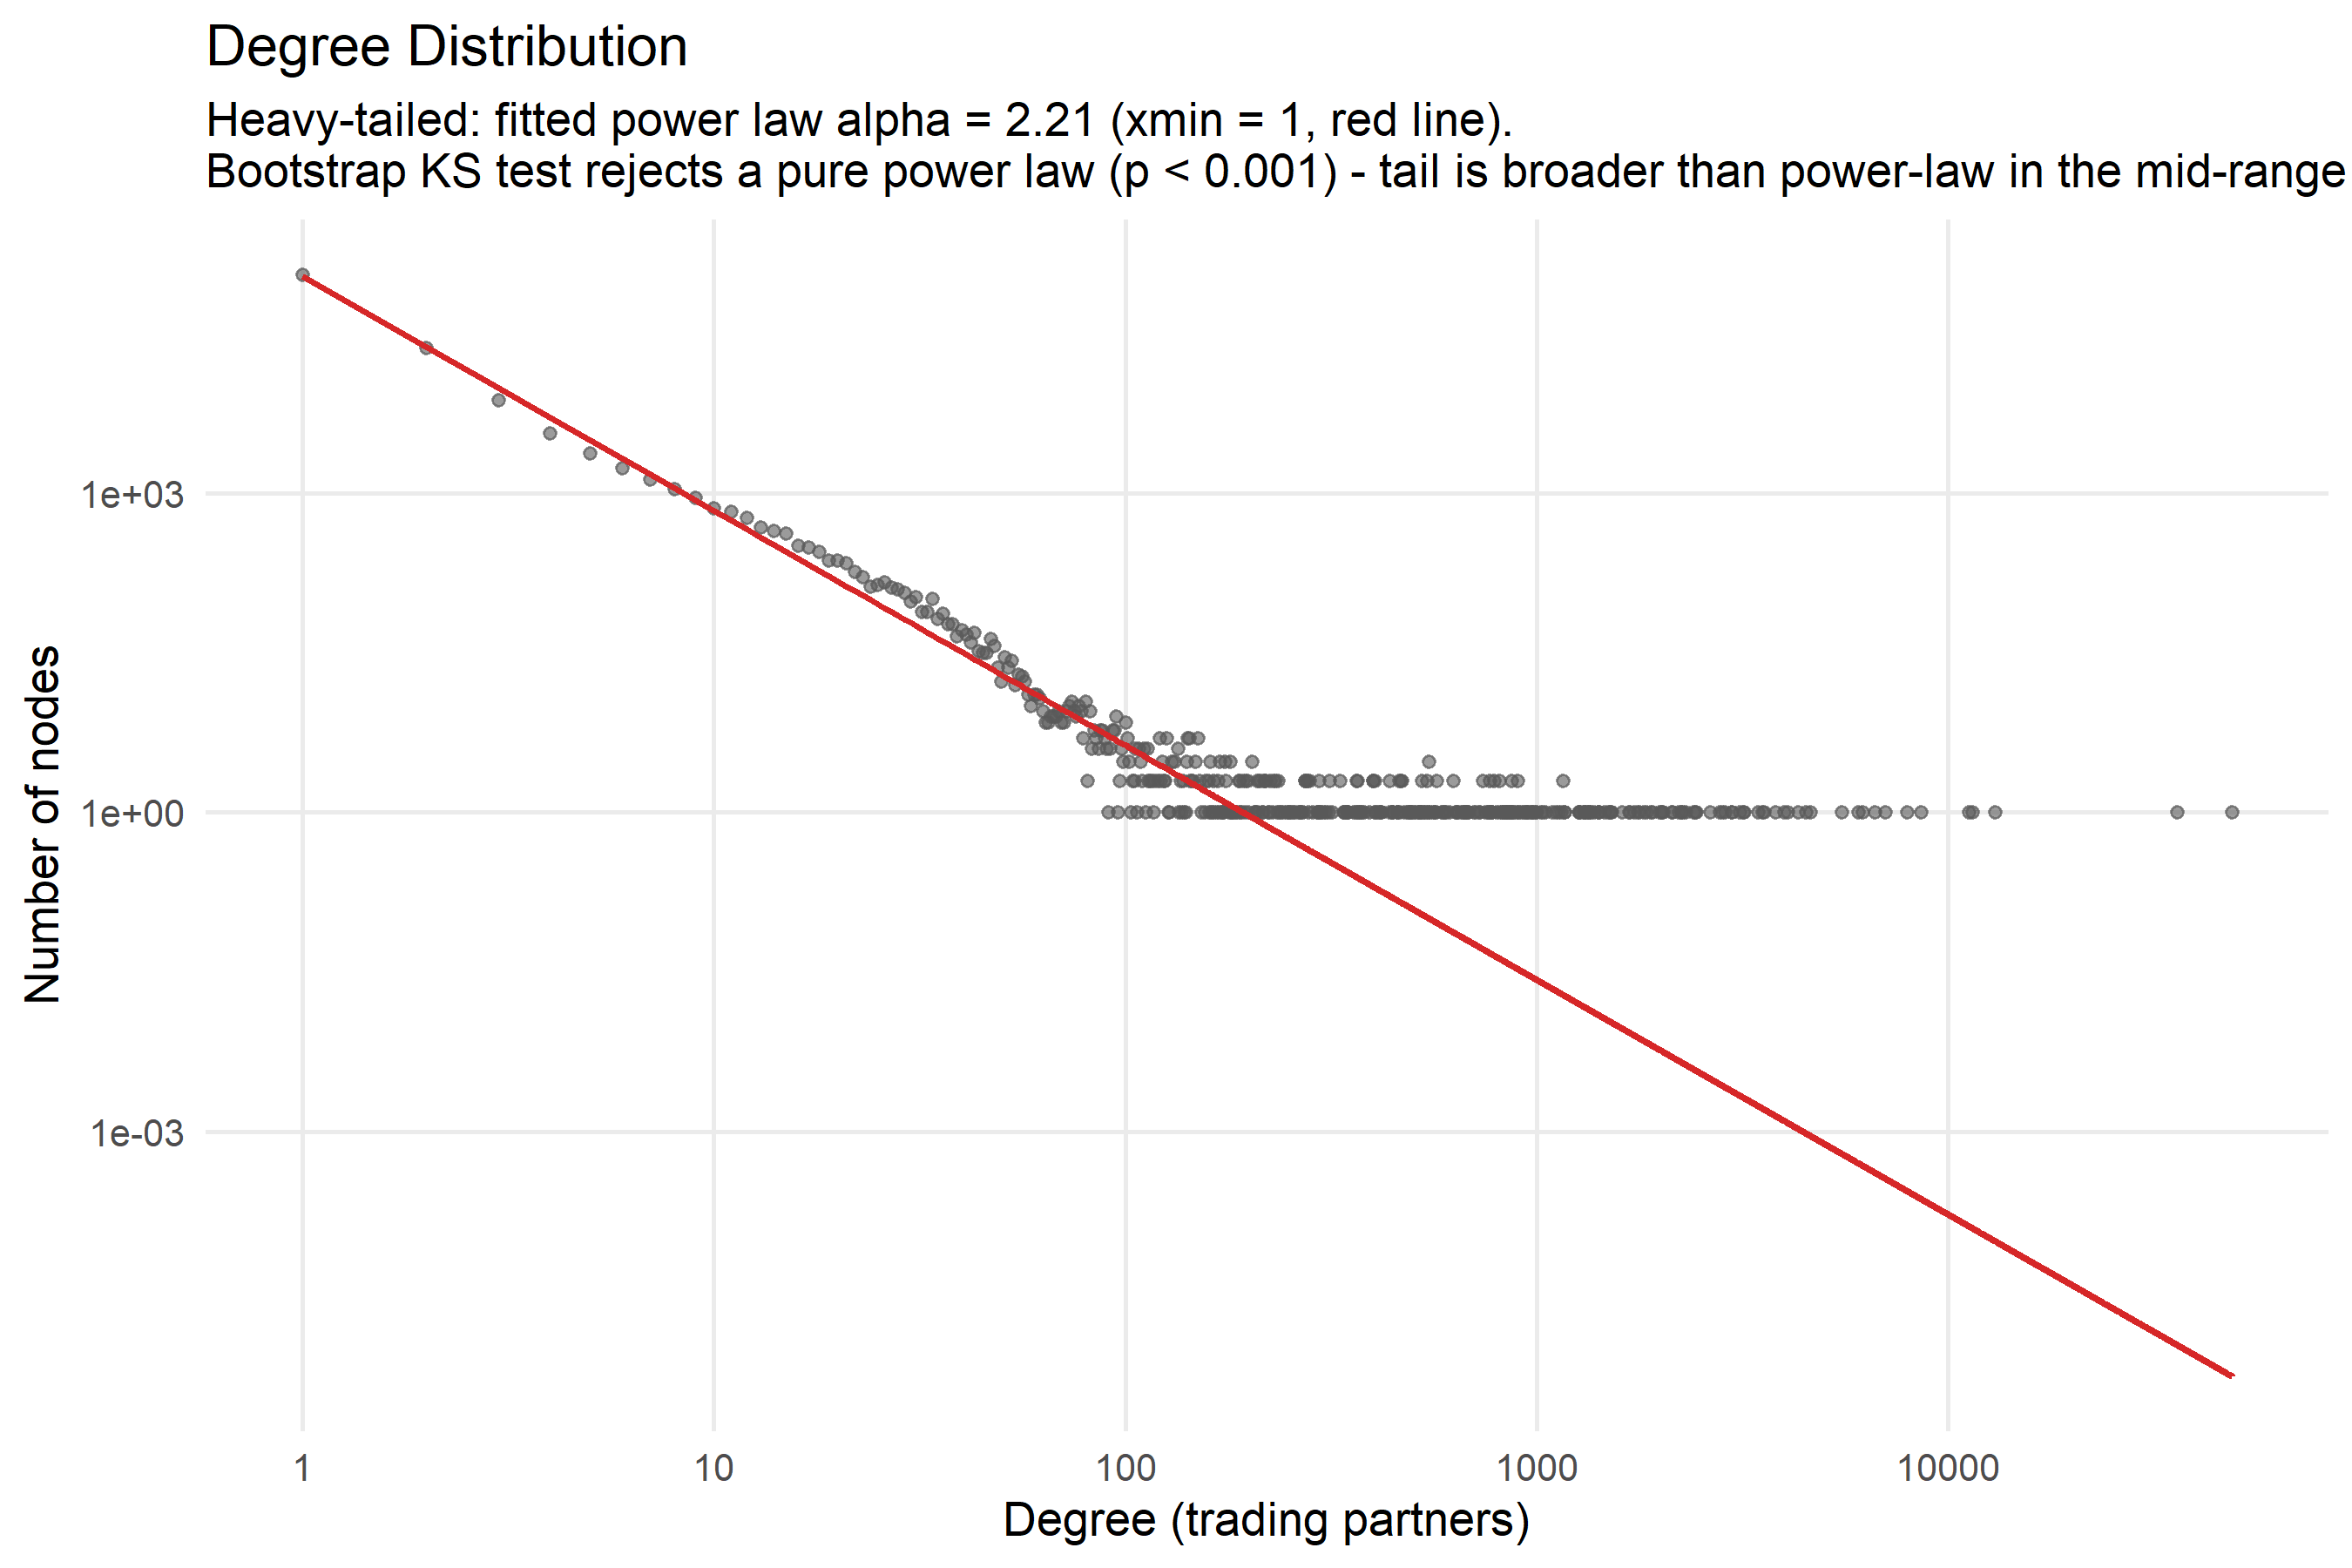
\includegraphics[width=\linewidth]{fig_temporal.png}
  \caption{Monthly invoice volumes over the 2018--2022 study period.
           The post-2018 decline in sales records reflects system migration
           rather than reduced economic activity; purchase volumes remain stable.}
  \label{fig:temporal}
\end{figure}

\subsection{Transaction Graph Construction}

We model the EFRIS data as a directed, heterogeneous graph
$\mathcal{G} = (\mathcal{V}, \mathcal{E}, \mathcal{R})$ where:

\begin{itemize}
  \item $\mathcal{V}$ is the set of all entities (taxpayers and counterparties),
        $|\mathcal{V}| = 30{,}173$.
  \item $\mathcal{E}$ is the set of directed, aggregated transaction edges,
        $|\mathcal{E}| = 144{,}426$.
  \item $\mathcal{R} = \{\texttt{sells\_to},\, \texttt{buys\_from}\}$ are the
        two relation types, corresponding to sales (73,827 edges) and purchase
        (70,599 edges) relationships respectively.
\end{itemize}

Multiple invoices between the same buyer--seller pair in the same relation
direction are aggregated into a single edge with attributes including total
transaction amount, total VAT, invoice count, and months active. Edge amounts
are log-transformed and IQR-normalised. The resulting graph is weakly connected
(one component) with a mean degree of 9.6, a maximum degree of 3,546, and a
mean clustering coefficient of 0.4918, indicating a highly heterogeneous,
scale-free-like topology typical of economic networks.

\subsection{Taxpayer Features}

Of the 30,173 nodes, 614 are \emph{registered taxpayers} with known identities;
the remainder are counterparties (suppliers or buyers) appearing only in
transaction records. Feature engineering is restricted to the 614 taxpayer
nodes, yielding a $614 \times 26$ feature matrix. Features are constructed in
three groups:

\begin{enumerate}
  \item \textbf{Sales-side features} (10): total sales, total output VAT,
        invoice count, unique buyers, average/variance/median invoice value,
        activity code diversity, and months/years active as seller.
  \item \textbf{Purchase-side features} (10): analogous features computed from
        the purchase invoice stream.
  \item \textbf{Derived ratio features} (6): output-to-input VAT ratio,
        purchase-to-sales ratio, total unique trading partners, combined average
        invoice value, combined variance, and combined months active.
\end{enumerate}

Missing values arising from taxpayers with only one stream (83 purchase-only
taxpayers; no sales-only taxpayers) are imputed with zero. Infinite ratios
(arising from zero denominators) are similarly zeroed. The feature distribution
is strongly right-skewed; log-transformations are applied in the GNN pipeline.

\subsection{Problem Formulation}

\textbf{Unsupervised anomaly detection:} Given the graph $\mathcal{G}$ and the
taxpayer feature matrix $\mathbf{X} \in \mathbb{R}^{614 \times 26}$, compute a
per-taxpayer anomaly score $s_i \in [0,1]$ such that entities whose feature
profiles or network positions deviate substantially from the majority receive
high scores. Since no fraud labels exist, models are evaluated through:
(i) mutual complementarity of scores, (ii) interpretability of flagged cases,
(iii) temporal validation against burst-activity patterns, and
(iv) robustness across contamination thresholds.

% ============================================================
\section{Methodology}
\label{sec:method}

Our framework consists of three independently trained unsupervised models
whose outputs are combined via a consensus ensemble. Figure~\ref{fig:pipeline}
provides a schematic overview.

\begin{figure}[htb]
  \centering
  % Pipeline schematic (text-based table approximation)
  \small
  \renewcommand{\arraystretch}{1.3}
  \begin{tabular}{|c|}
    \hline
    \textbf{EFRIS Raw Data}\\
    Sales \& Purchase Invoices (2018--2022)\\
    \hline
    $\downarrow$ Preprocessing \& Feature Engineering\\
    \hline
    \begin{tabular}{c@{\quad}c}
      \textbf{Tabular Features} & \textbf{Transaction Graph}\\
      $614 \times 26$ matrix & 30,173 nodes, 144,426 edges
    \end{tabular}\\
    \hline
    $\downarrow$\quad\quad\quad\quad$\downarrow$\quad\quad\quad\quad$\downarrow$\\
    \hline
    \begin{tabular}{c@{\;\;}c@{\;\;}c}
      \textbf{IF} & \textbf{RGCN} & \textbf{GAT}\\
      Feature & Relational & Attention\\
      outliers & structure & embeddings
    \end{tabular}\\
    \hline
    $\downarrow$ Consensus Ensemble (flagged by $\geq 2$ models)\\
    \hline
    \textbf{27 High-Confidence Suspects}\\
    \hline
  \end{tabular}
  \caption{Overview of the three-model ensemble framework. Each model detects
           a distinct anomaly dimension; consensus cases are flagged by at least
           two models.}
  \label{fig:pipeline}
\end{figure}

\subsection{Extended Isolation Forest (IF)}

Isolation Forest \cite{liu2008isolation} detects anomalies by measuring how
quickly a data point can be isolated through recursive random partitioning.
Points requiring fewer splits are more anomalous. We use the Extended Isolation
Forest (EIF) \cite{hariri2019extended} implemented via the \texttt{isotree}
R package \cite{cortes2021isotree}, which uses hyperplane cuts in multiple
dimensions to reduce the diagonal bias of the original algorithm.

Hyperparameters are selected via an 18-configuration grid search over
\texttt{ntrees} $\in \{100, 300, 500\}$,
\texttt{sample\_size} $\in \{64, 128, 256\}$, and
\texttt{ndim} $\in \{1, 2\}$.
Selection criterion is the configuration maximising score standard deviation
(discrimination power). Convergence analysis (Figure~\ref{fig:if_convergence})
shows that Spearman rank correlation with the 500-tree model exceeds 0.99 at
approximately 200 trees, validating the adequacy of the chosen tree count.

\begin{figure}[htb]
  \centering
  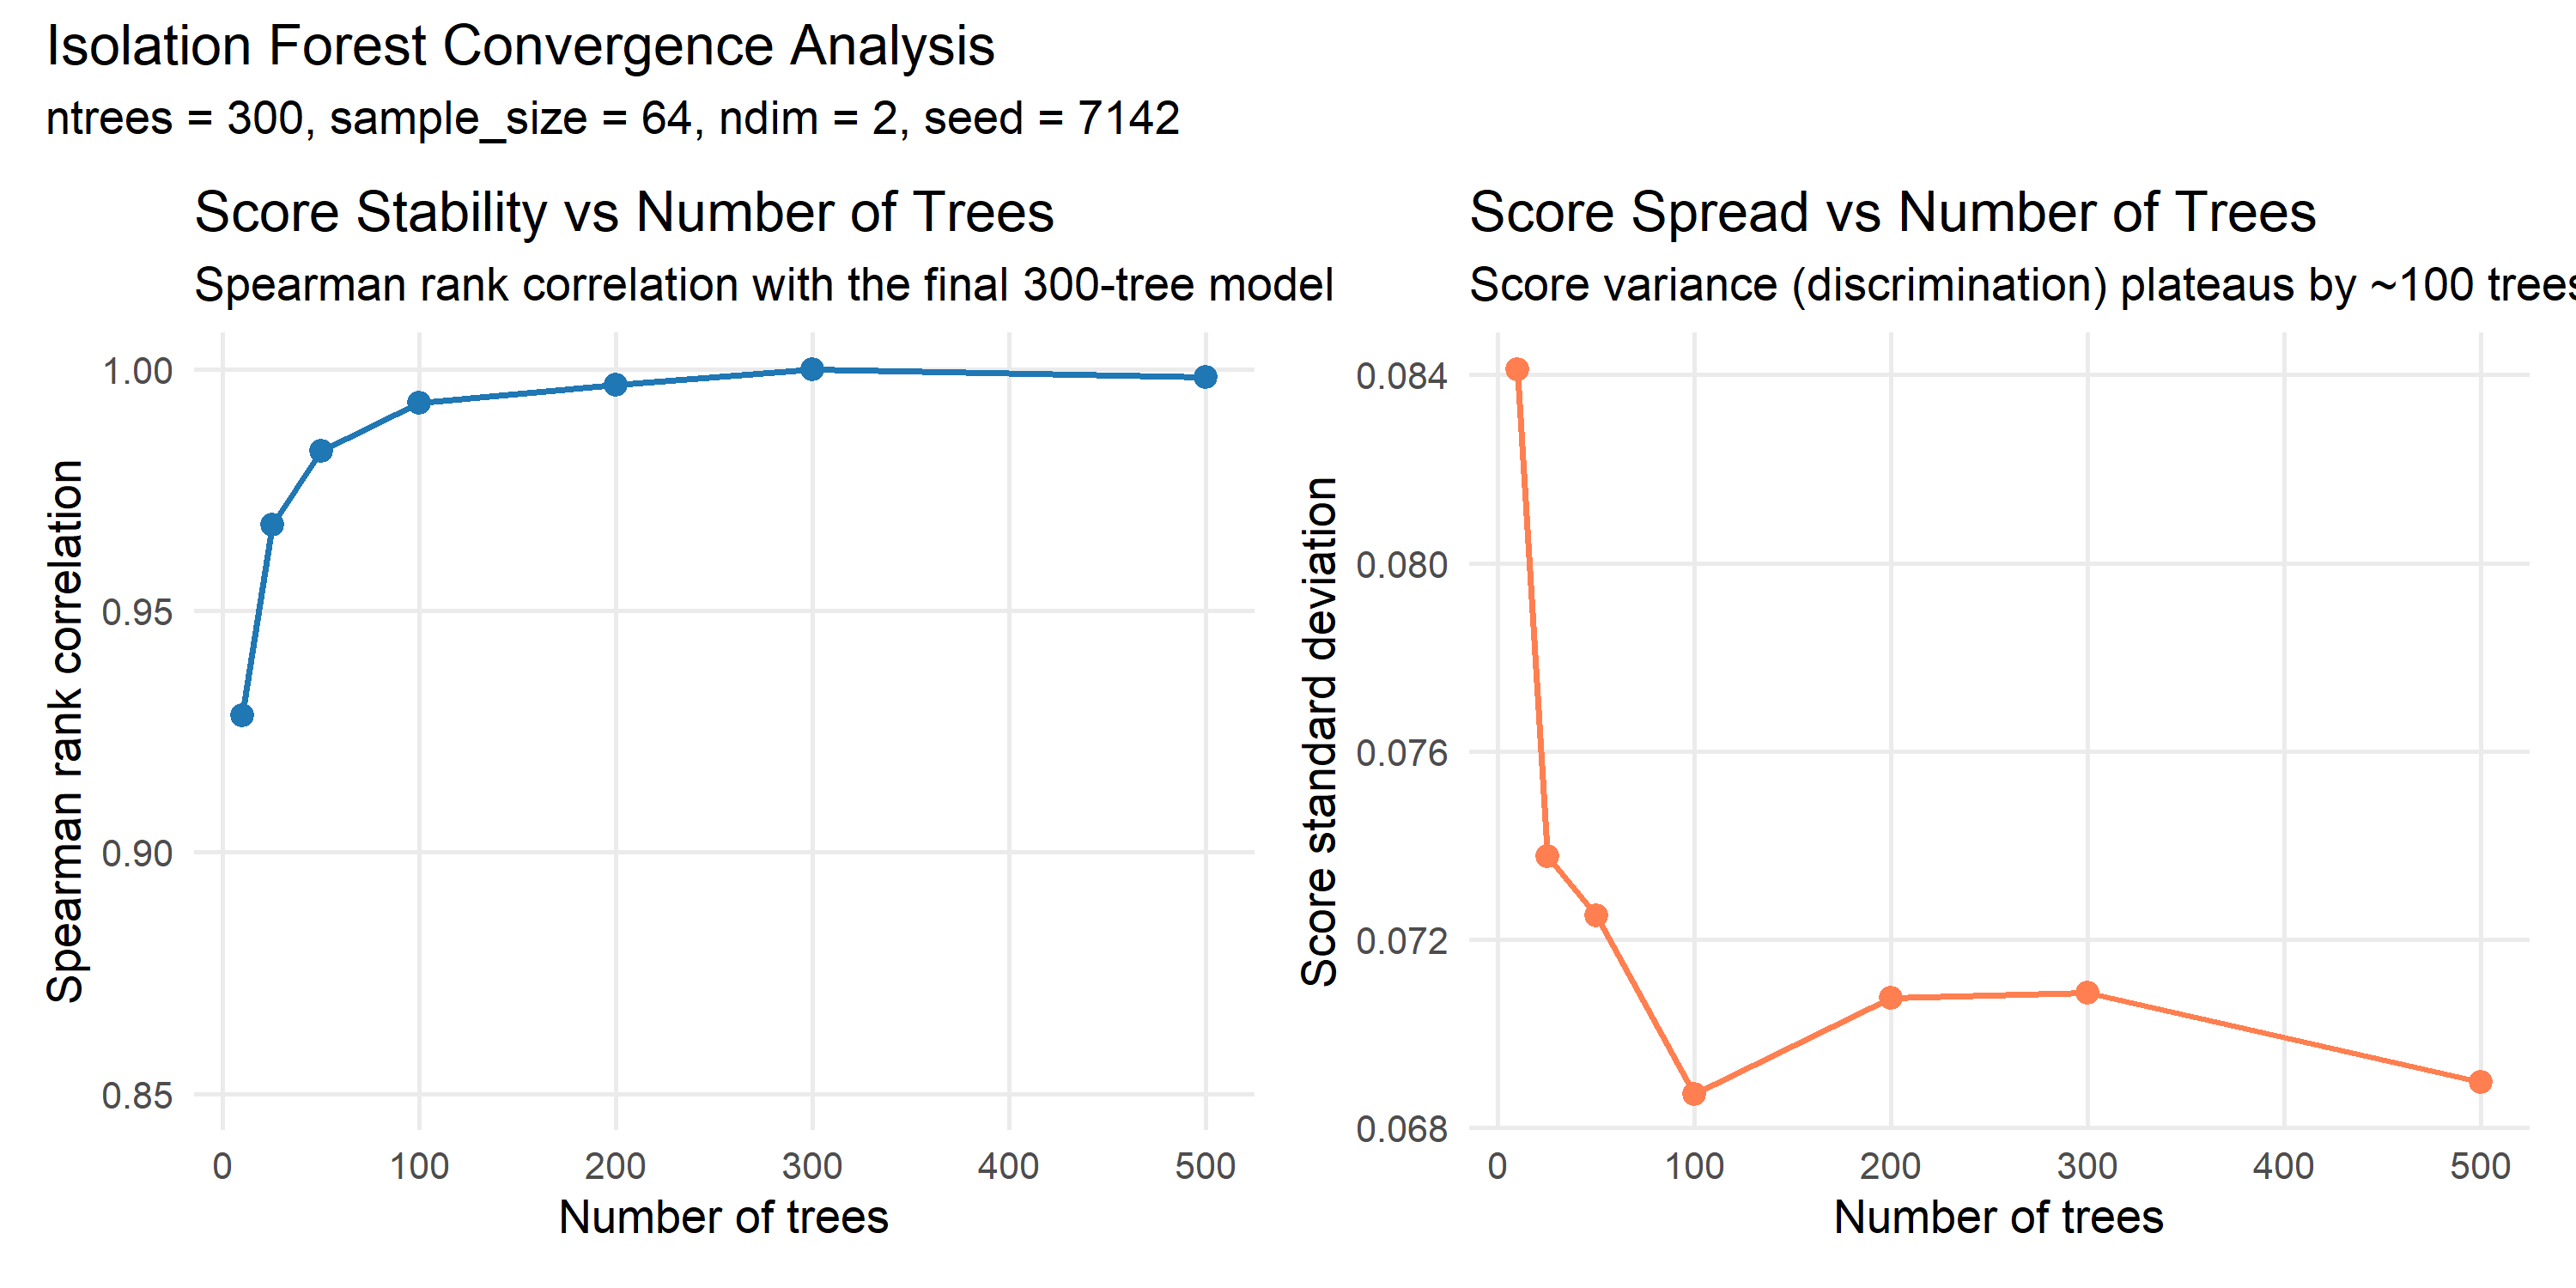
\includegraphics[width=\linewidth]{fig_if_convergence.png}
  \caption{Isolation Forest convergence analysis. Left: Spearman rank
           correlation with the 500-tree reference model crosses the 0.99
           threshold at $\approx$200 trees. Right: score discrimination (std.\ dev.)
           stabilises after 100 trees.}
  \label{fig:if_convergence}
\end{figure}

Anomaly scores are normalised to $[0, 1]$ and the top 10\% (62 taxpayers)
are designated as IF-flagged. Feature-importance analysis computes the mean
absolute z-score deviation of flagged taxpayers from the normal group for each
feature, identifying purchase-amount variance, sales-amount variance,
output/input VAT ratio, and purchase-to-sales ratio as the primary drivers
(Figure~\ref{fig:feat_importance}).

\subsection{Relational Graph Convolutional Network (RGCN)}

The RGCN \cite{schlichtkrull2018modeling} extends GCNs to heterogeneous graphs
with multiple relation types via basis decomposition. Node features from the
26-dimensional taxpayer feature matrix are concatenated with zero vectors for
counterparty nodes, yielding an initial feature matrix
$\mathbf{X} \in \mathbb{R}^{30173 \times 26}$.

\textbf{Architecture.} Two RGCN layers map from 26 input dimensions to 64
hidden dimensions and then to a 32-dimensional embedding, with basis
decomposition using $B = 2$ bases and 0.3 dropout. A two-layer
link-prediction decoder maps concatenated source--destination embedding pairs
to a scalar edge-existence score.

\textbf{Training.} The model is trained self-supervisedly on a
\emph{link-prediction} task: 15\% of edges are randomly masked and the model
is trained to distinguish masked (positive) edges from randomly sampled
negative edges using binary cross-entropy loss. Training runs for 150 epochs
(Adam optimiser, $\text{lr}=0.005$, weight decay $10^{-5}$, gradient clipping
at 1.0). Final training loss converges to 0.0807 in approximately 30.9~seconds.

\textbf{Anomaly scoring.} After training, per-node anomaly scores are computed
as the mean squared reconstruction error averaged across all incident edges:
\begin{equation}
  s_i^{\text{RGCN}} = \frac{1}{|\mathcal{N}(i)|}
    \sum_{j \in \mathcal{N}(i)} (1 - \hat{p}_{ij})^2,
\end{equation}
where $\hat{p}_{ij} = \sigma(\text{decoder}(\mathbf{z}_i, \mathbf{z}_j))$ is
the predicted link probability and $\mathcal{N}(i)$ is the set of neighbours
of node $i$. Nodes whose edge reconstructions are systematically poor receive
high anomaly scores, indicating unusual relational structure.

\subsection{Graph Attention Network (GAT)}

The GAT \cite{velickovic2018graph} replaces fixed spectral aggregation with
learnable, per-edge attention weights, allowing the model to focus on the most
informative neighbours during message passing.

\textbf{Architecture.} Two GAT layers with 32 hidden dimensions and 4 attention
heads (concatenated) in the first layer, collapsing to 32 output dimensions in
the second layer, with 0.3 dropout throughout.

\textbf{Training.} The same link-prediction pretraining paradigm is used. To
handle the large graph, 25\% of edges are sampled each epoch as positive
examples, with an equal number of negative samples drawn via corruption.
Training runs for 150 epochs with the same optimiser settings as RGCN. Final
training loss is 0.2505 in approximately 70.8~seconds.

\textbf{Anomaly scoring.} After training, node embeddings
$\mathbf{z}_i \in \mathbb{R}^{32}$ are extracted. $K$-means clustering is
applied to the full embedding matrix with $k$ selected by maximising silhouette
score over $k \in \{3, 5, 7, 10\}$. The optimal $k = 7$ achieves
silhouette $= 0.697$. Each node's anomaly score is its normalised distance to
its nearest cluster centroid:
\begin{equation}
  s_i^{\text{GAT}} = \frac{d({\mathbf{z}}_i, c_{k(i)}) - d_{\min}}{d_{\max} - d_{\min}},
\end{equation}
where $c_{k(i)}$ is the centroid of node $i$'s assigned cluster.

\subsection{Ensemble Consensus}

Because the three models capture distinct anomaly dimensions (tabular feature
outliers, relational structure anomalies, and embedding isolation respectively),
their scores are largely uncorrelated. We flag a taxpayer as a consensus
case if and only if it appears in the top 10\% of at least two model score
distributions:

\begin{equation}
  \text{consensus}_i = \mathbb{1}\left[
    \sum_{m \in \{\text{IF, RGCN, GAT}\}}
    \mathbb{1}[s_i^m \geq Q_{0.9}^m] \geq 2
  \right],
\end{equation}
where $Q_{0.9}^m$ is the 90th percentile of model $m$'s score distribution.
The 10\% flagging threshold per model is chosen to balance recall (capture
enough suspects for scrutiny) with the operational cost of false positives in
an audit context. All experiments use global seed 7142 for full reproducibility
across both R and Python components.

% ============================================================
\section{Experimental Results}
\label{sec:results}

\subsection{Network Topology}

The EFRIS transaction graph has properties typical of real-world economic
networks. Degree distribution follows an approximate power law
(Figure~\ref{fig:community}), with the majority of nodes having degree 1
(single-transaction counterparties) and a small hub population; the most
connected node has degree 3,546. Louvain community detection
\cite{blondel2008fast} identifies 16 communities (modularity $= 0.347$), with
the five largest containing 6,494; 5,638; 4,366; 1,854; and 1,836 nodes
respectively. Registered taxpayers are distributed across all 16 communities,
indicating broad participation throughout the transaction ecosystem.

\begin{figure}[htb]
  \centering
  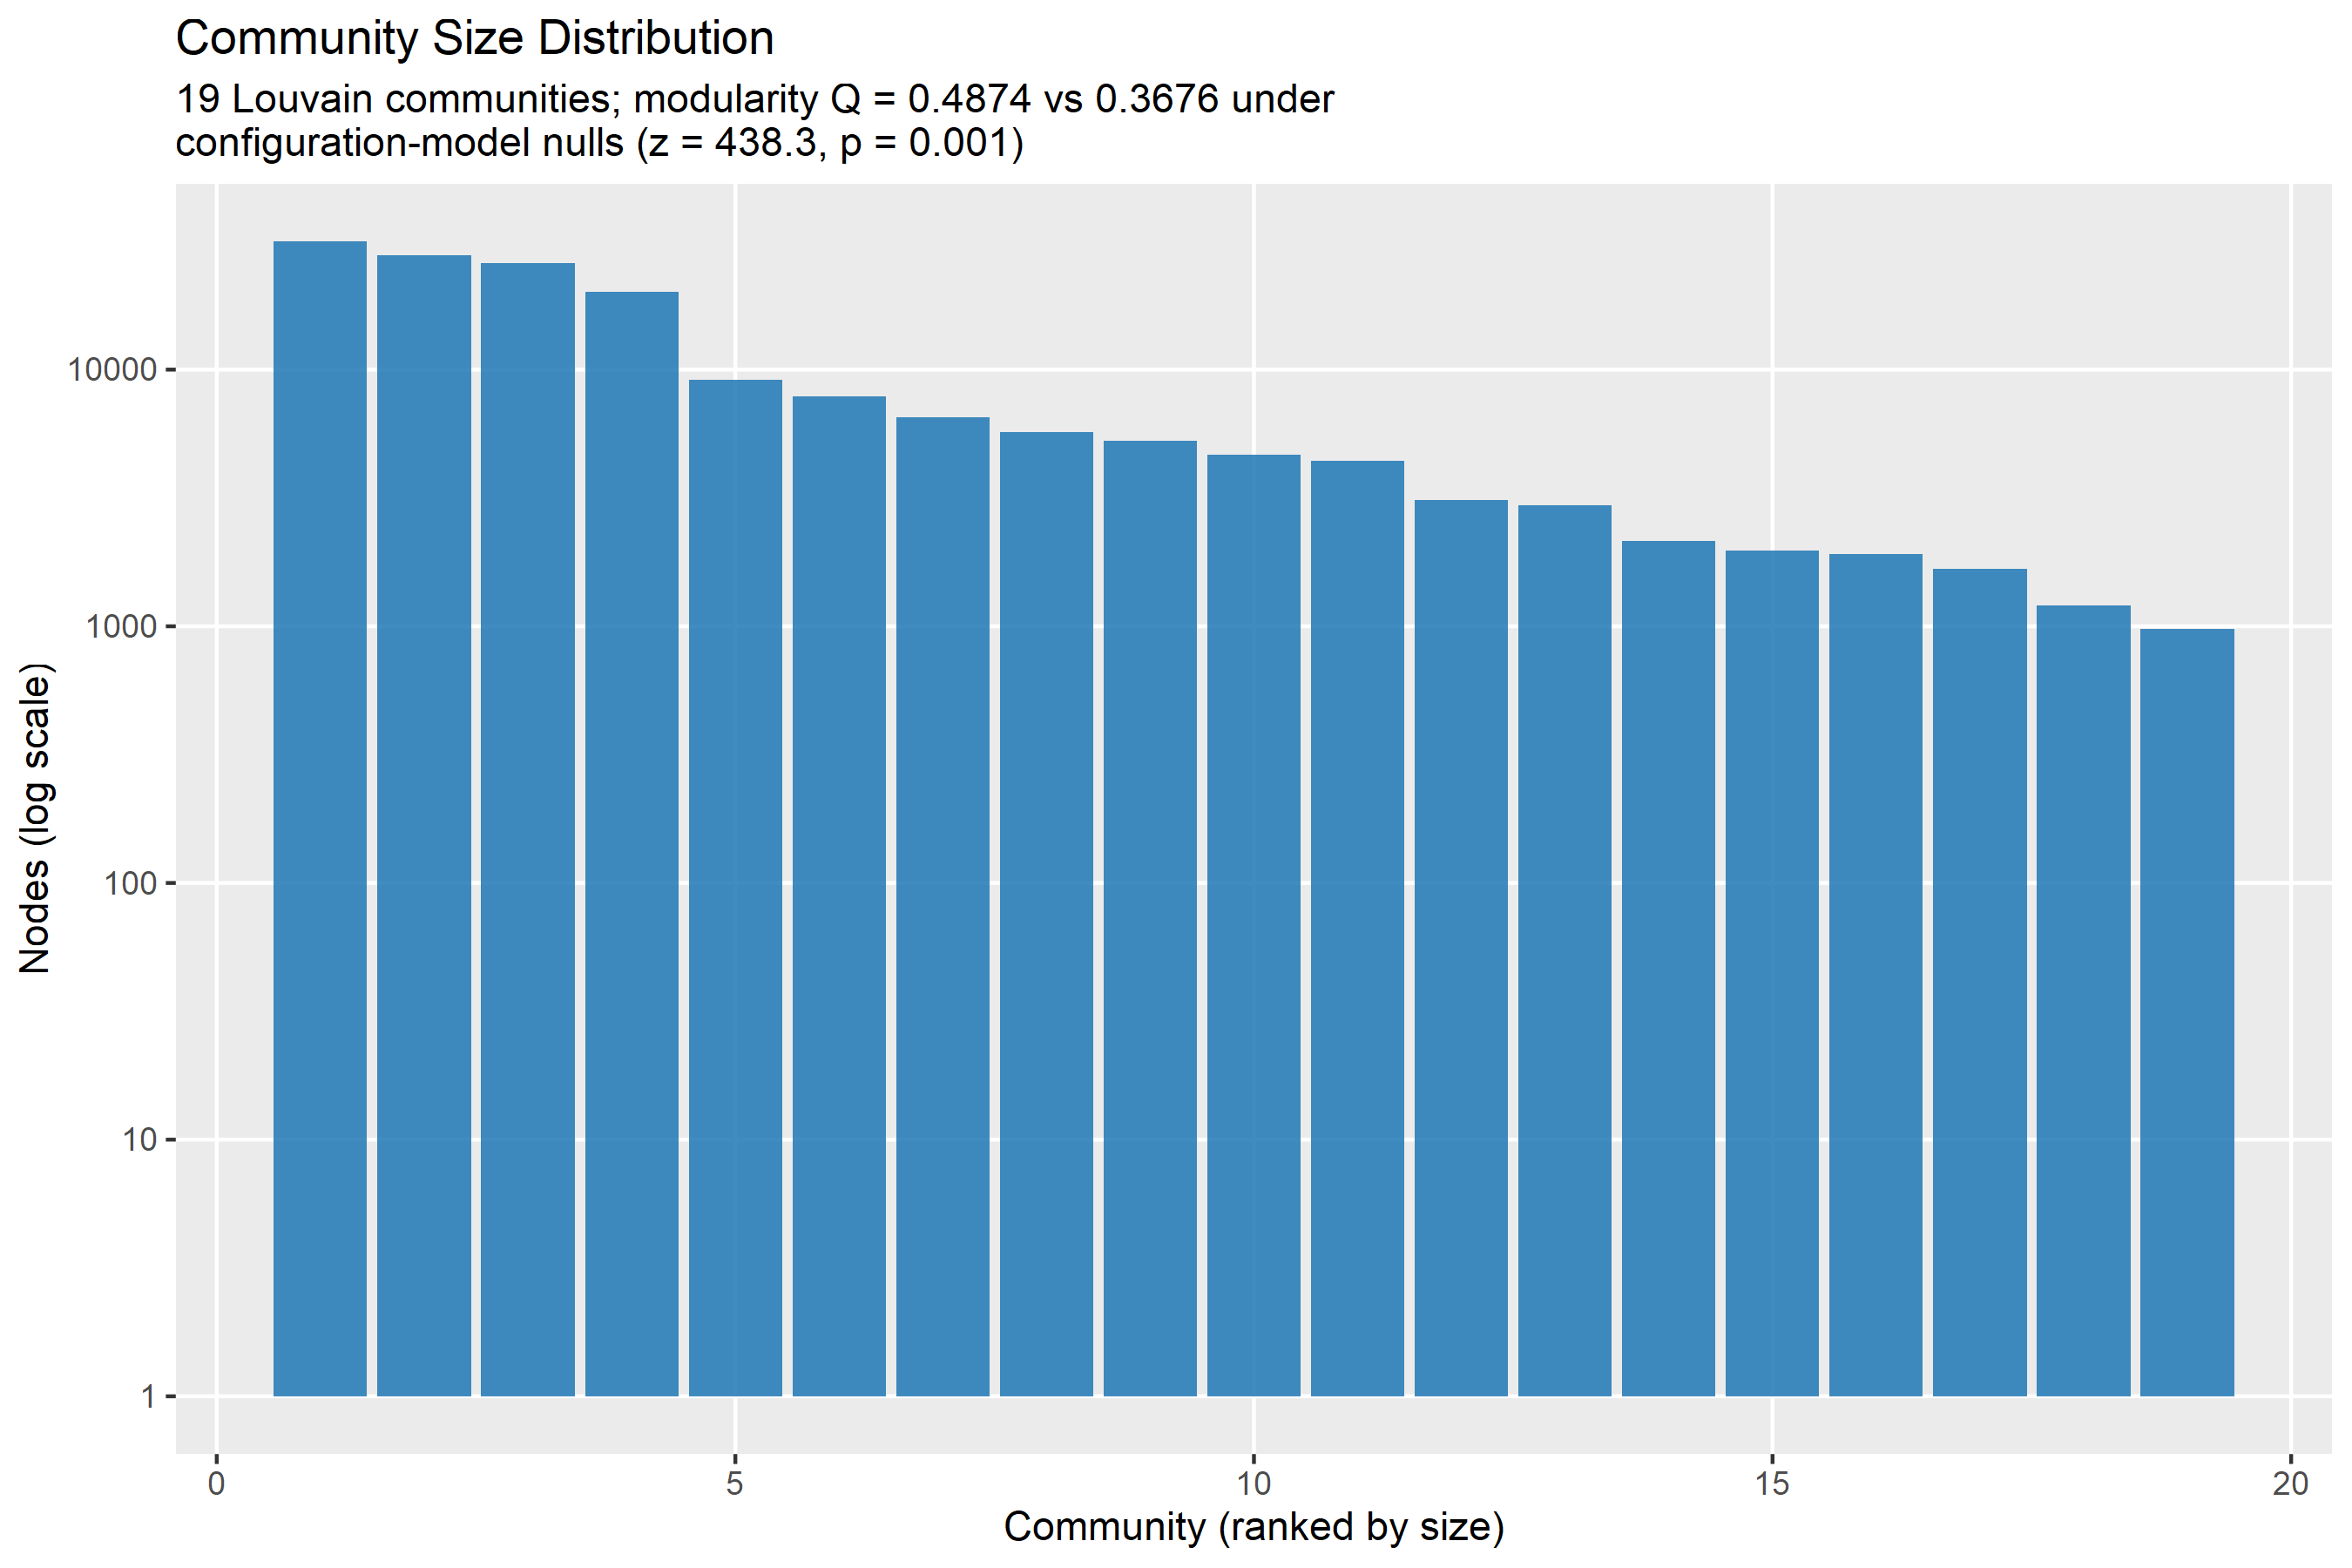
\includegraphics[width=\linewidth]{fig_community.png}
  \caption{Community size distribution from Louvain detection (16 communities,
           modularity $= 0.347$). Taxpayers are distributed across all communities.}
  \label{fig:community}
\end{figure}

\subsection{Isolation Forest Results}

Figure~\ref{fig:if_scores} shows the distribution of IF anomaly scores.
The score distribution is right-skewed, with a long tail of high-score
taxpayers. The 90th-percentile threshold (0.62) cleanly separates the bulk of
normal taxpayers from the 62 flagged cases. Feature importance analysis
(Figure~\ref{fig:feat_importance}) identifies \texttt{var\_purchase\_value}
and \texttt{var\_sale\_value} as the top drivers, indicating that flagged
taxpayers exhibit unusual volatility in invoice amounts. The
\texttt{output\_input\_vat\_ratio} and \texttt{purchase\_to\_sales\_ratio}
rank third and fourth, highlighting extreme mismatches between tax collected
and tax claimed.

\begin{figure}[htb]
  \centering
  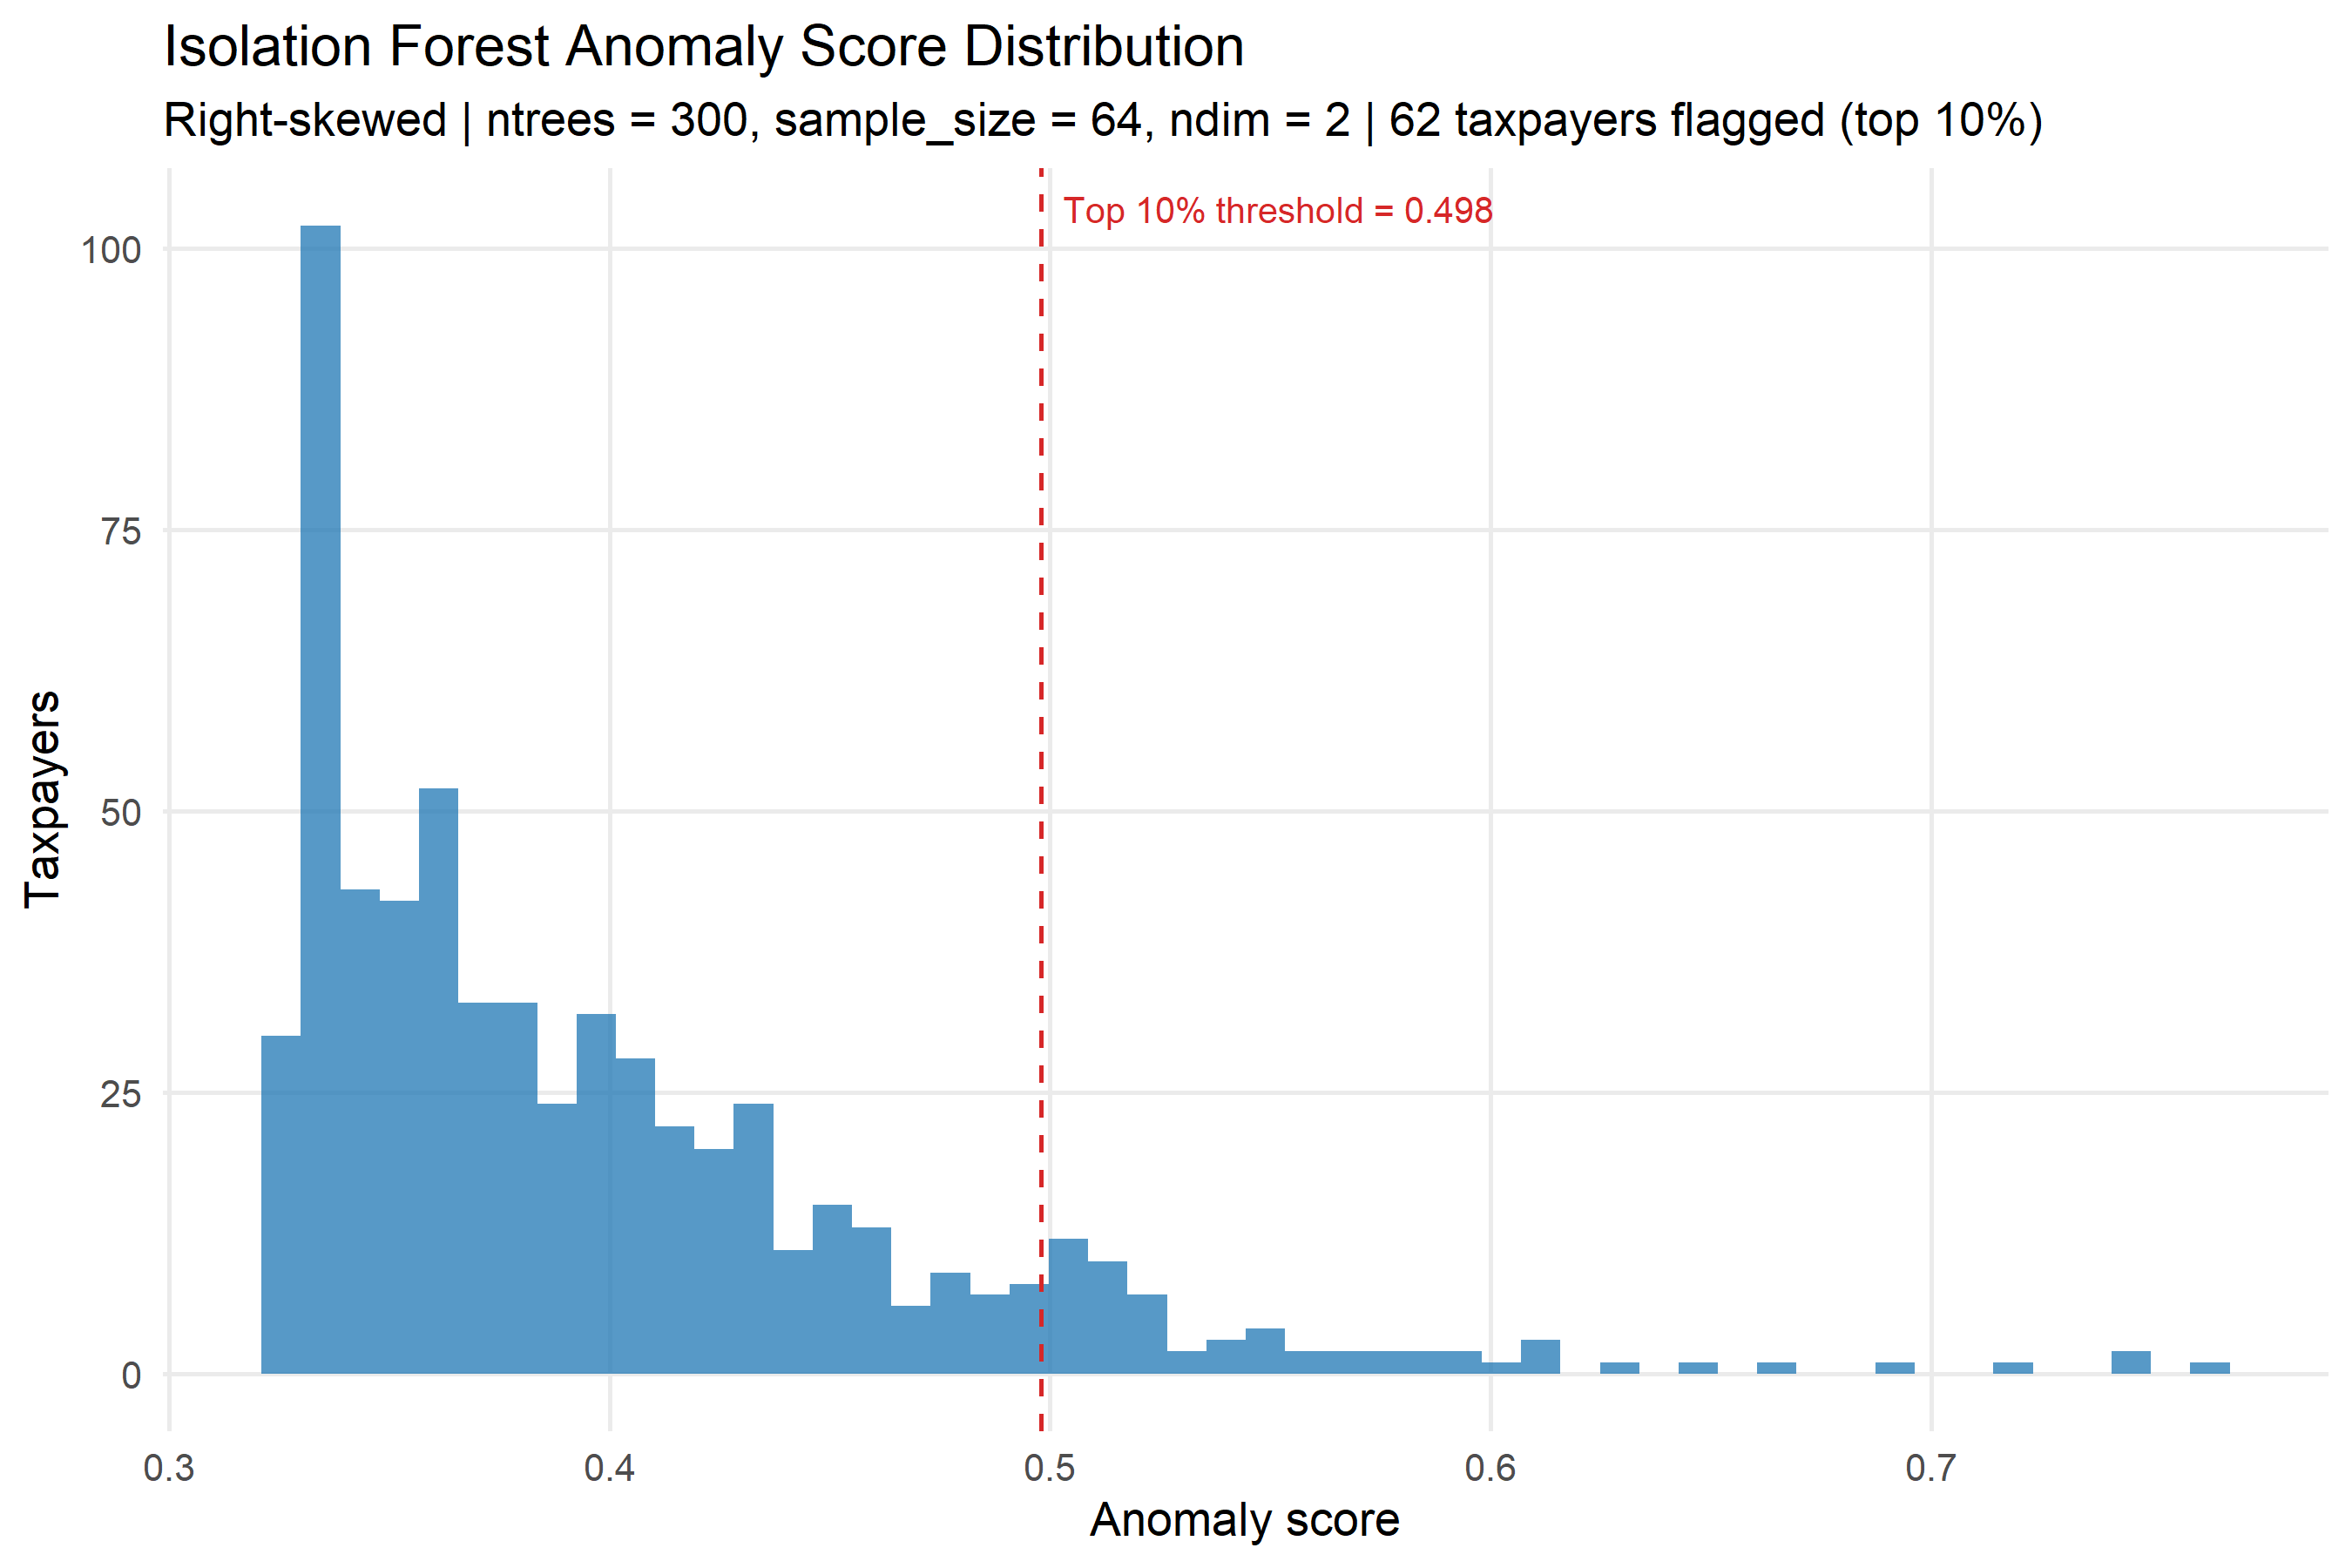
\includegraphics[width=\linewidth]{fig_if_scores.png}
  \caption{Isolation Forest anomaly score distribution across 614 taxpayers.
           The dashed red line marks the 90th-percentile flagging threshold.
           Sixty-two taxpayers fall above this threshold.}
  \label{fig:if_scores}
\end{figure}

\begin{figure}[htb]
  \centering
  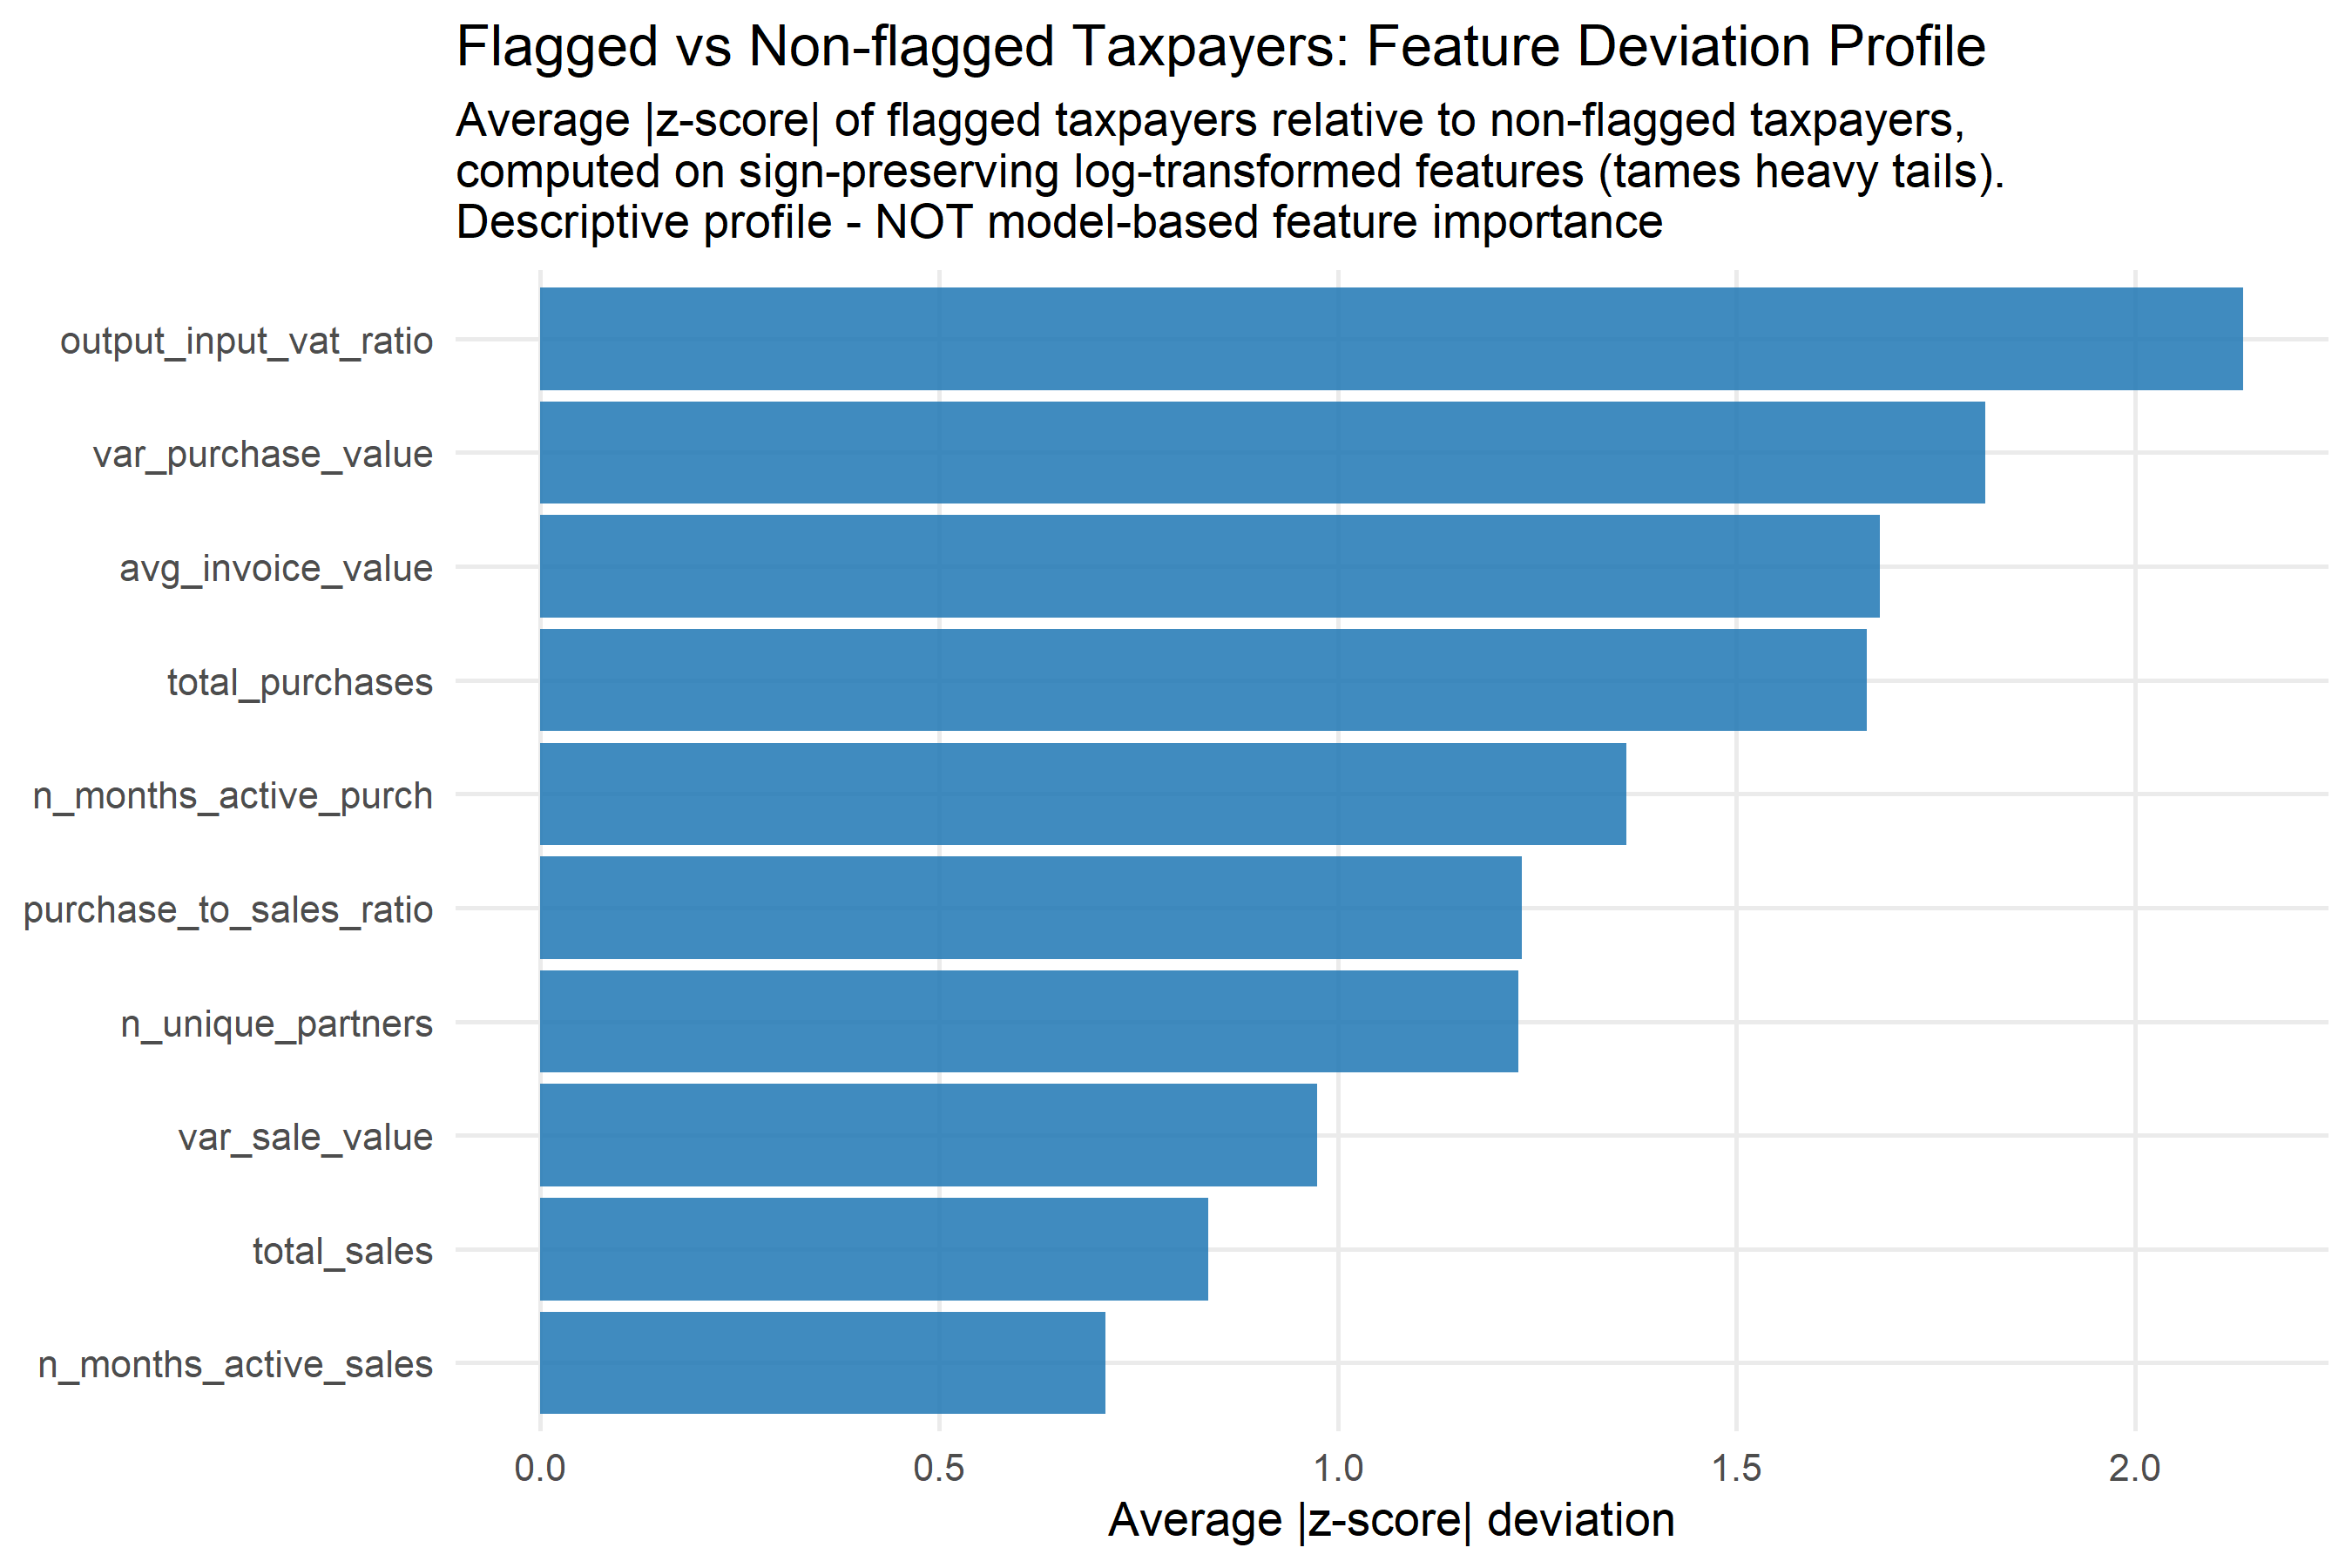
\includegraphics[width=\linewidth]{fig_feat_importance.png}
  \caption{Feature importance for Isolation Forest-flagged taxpayers, measured
           as mean absolute z-score deviation from the normal taxpayer group.
           Purchase and sales value variance dominate; VAT and purchase-to-sales
           ratios also contribute strongly.}
  \label{fig:feat_importance}
\end{figure}

Figure~\ref{fig:if_feature_space} places flagged and normal taxpayers in the
two key feature subspaces. The left panel (log sales vs.\ log purchases)
reveals a cluster of flagged taxpayers at extreme purchase levels relative to
sales. The right panel (purchase/sales ratio vs.\ output/input VAT ratio)
shows that flagged taxpayers occupy extreme corners of both axes simultaneously,
consistent with VAT manipulation.

\begin{figure}[htb]
  \centering
  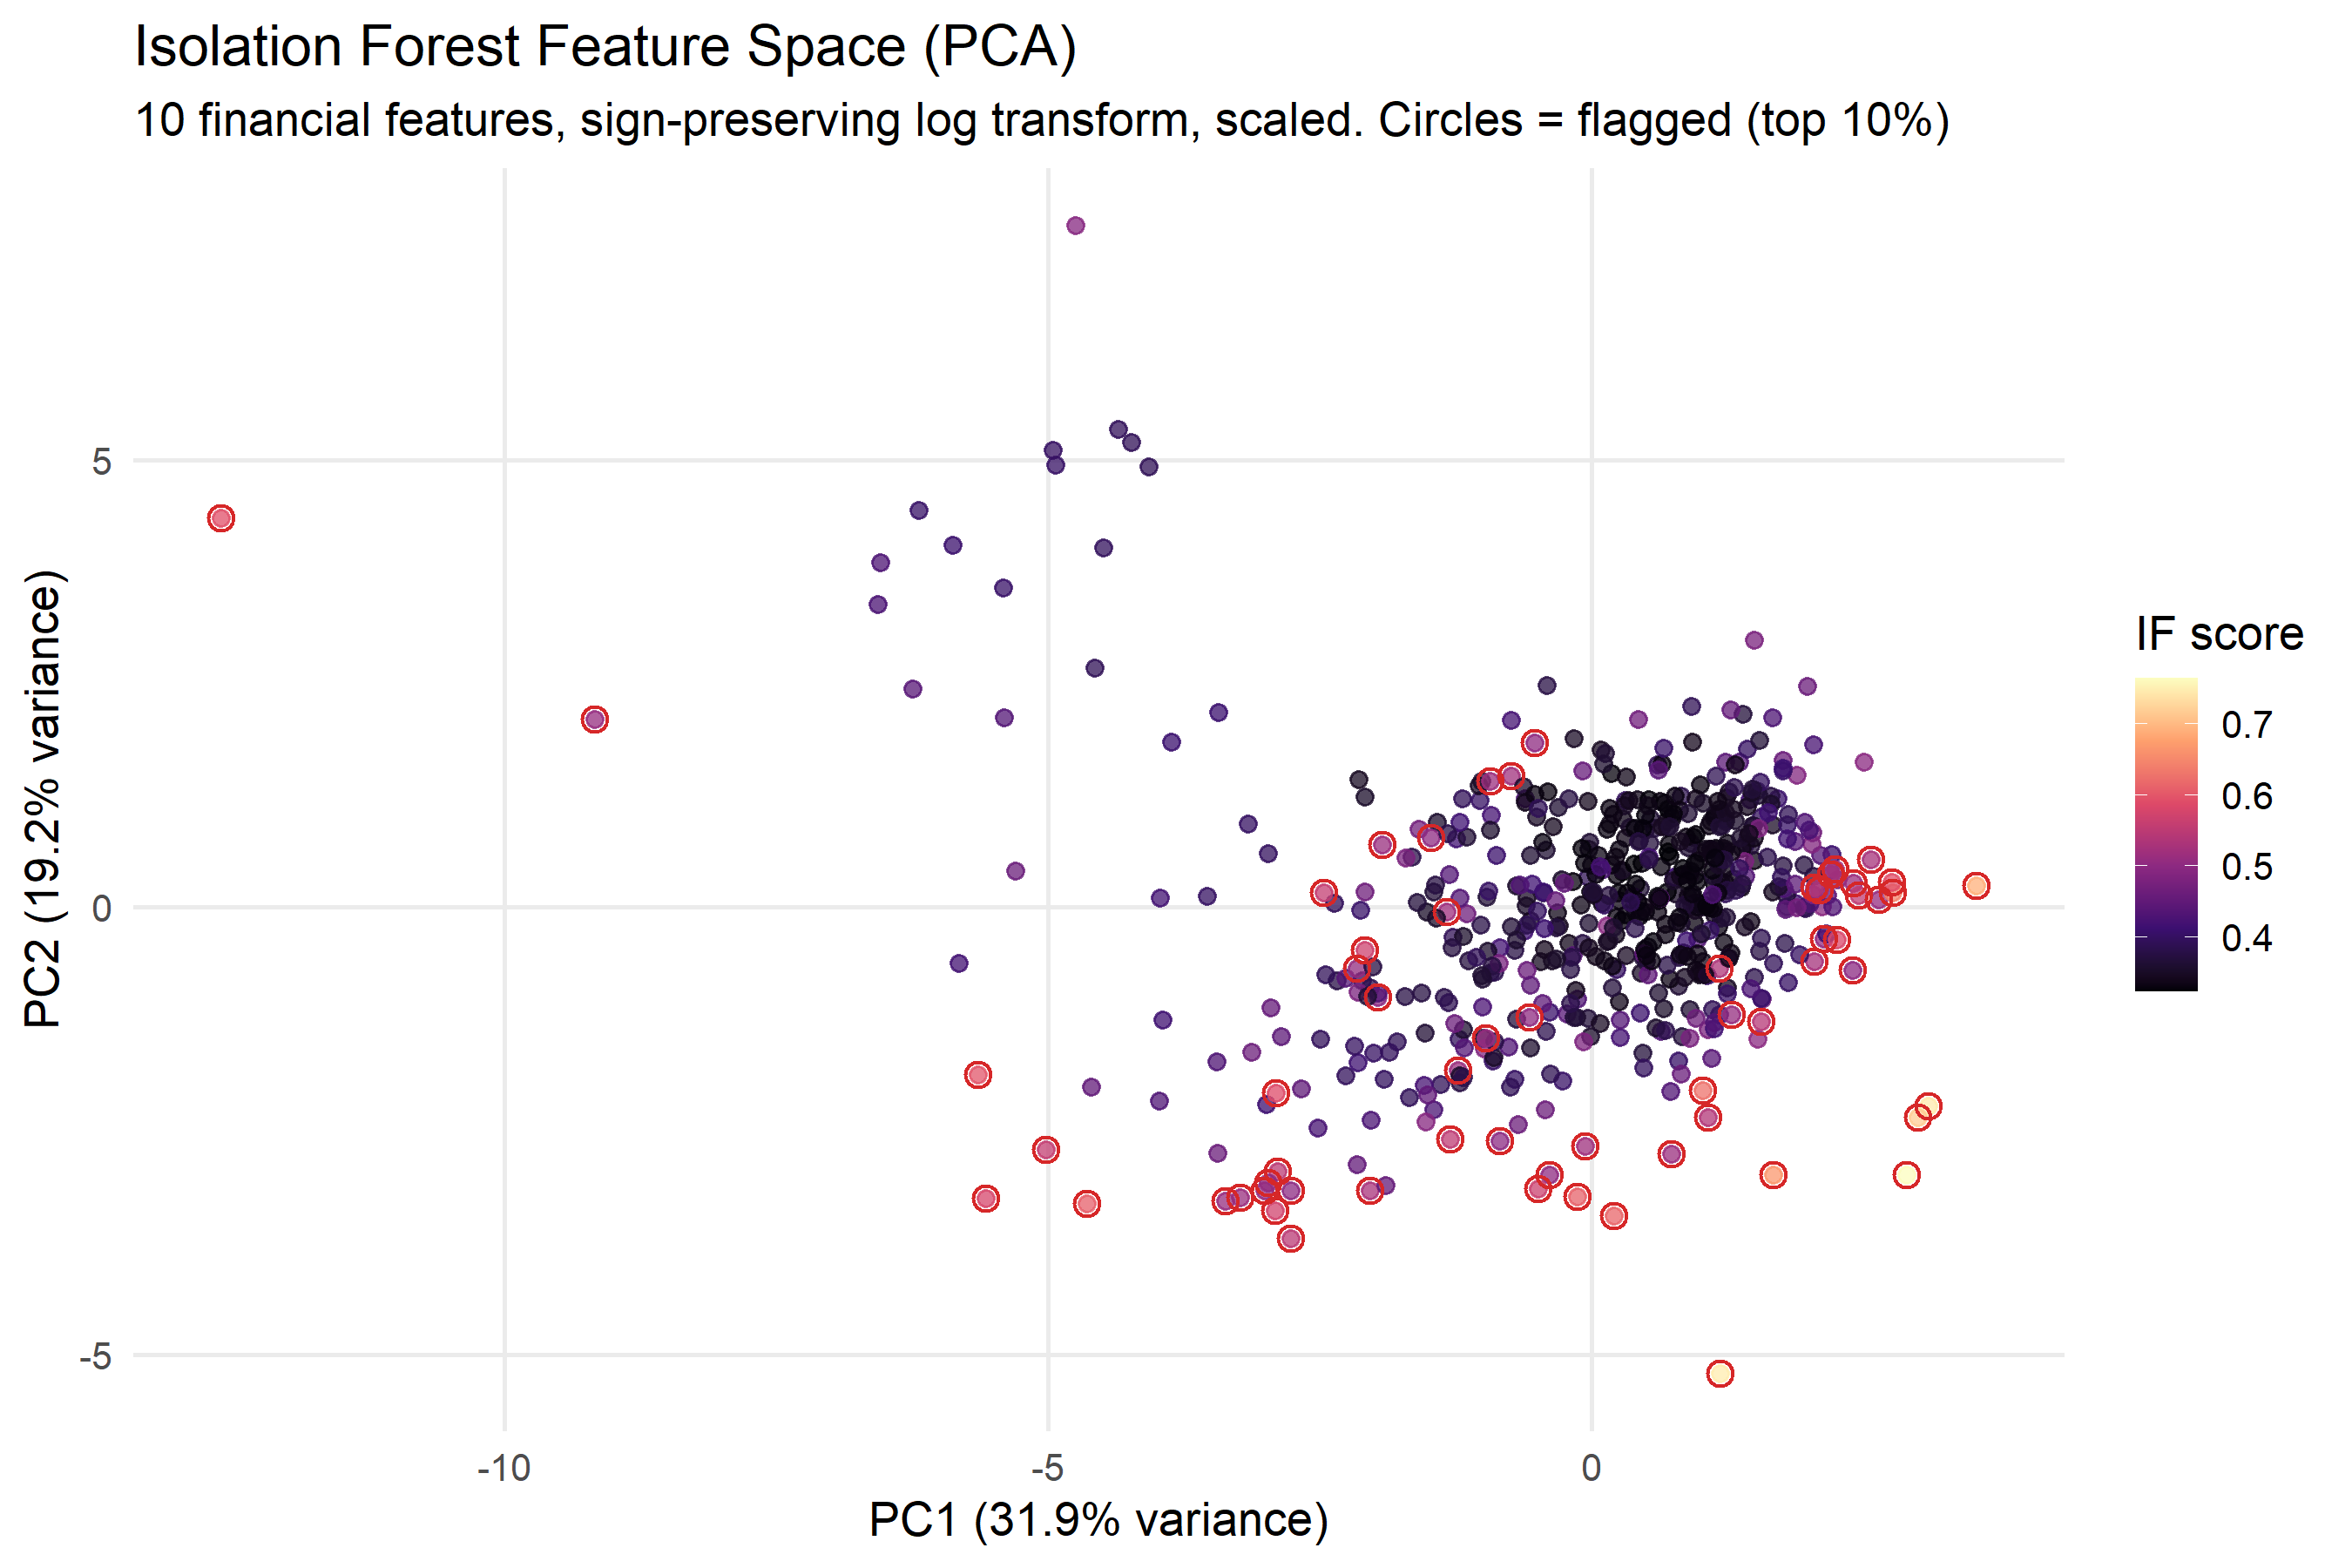
\includegraphics[width=\linewidth]{fig_if_feature_space.png}
  \caption{Isolation Forest-flagged taxpayers (red) vs.\ normal taxpayers
           (grey) in feature space. Left: log sales vs.\ log purchases. Right:
           purchase/sales ratio vs.\ output/input VAT ratio. Flagged taxpayers
           cluster at extremes of both axes.}
  \label{fig:if_feature_space}
\end{figure}

\subsection{GNN Training and Convergence}

Figure~\ref{fig:gnn_loss} presents training loss curves for both GNN models.
Both converge well within 150 epochs. RGCN achieves a substantially lower
final loss (0.0807) than GAT (0.2505), reflecting the benefit of modelling
the two relation types (\texttt{sells\_to}, \texttt{buys\_from}) explicitly
via basis-decomposed relation matrices. The higher GAT loss does not indicate
inferior anomaly detection; the two models operate on different detection
principles and their scores are, by design, near-orthogonal.

\begin{figure}[htb]
  \centering
  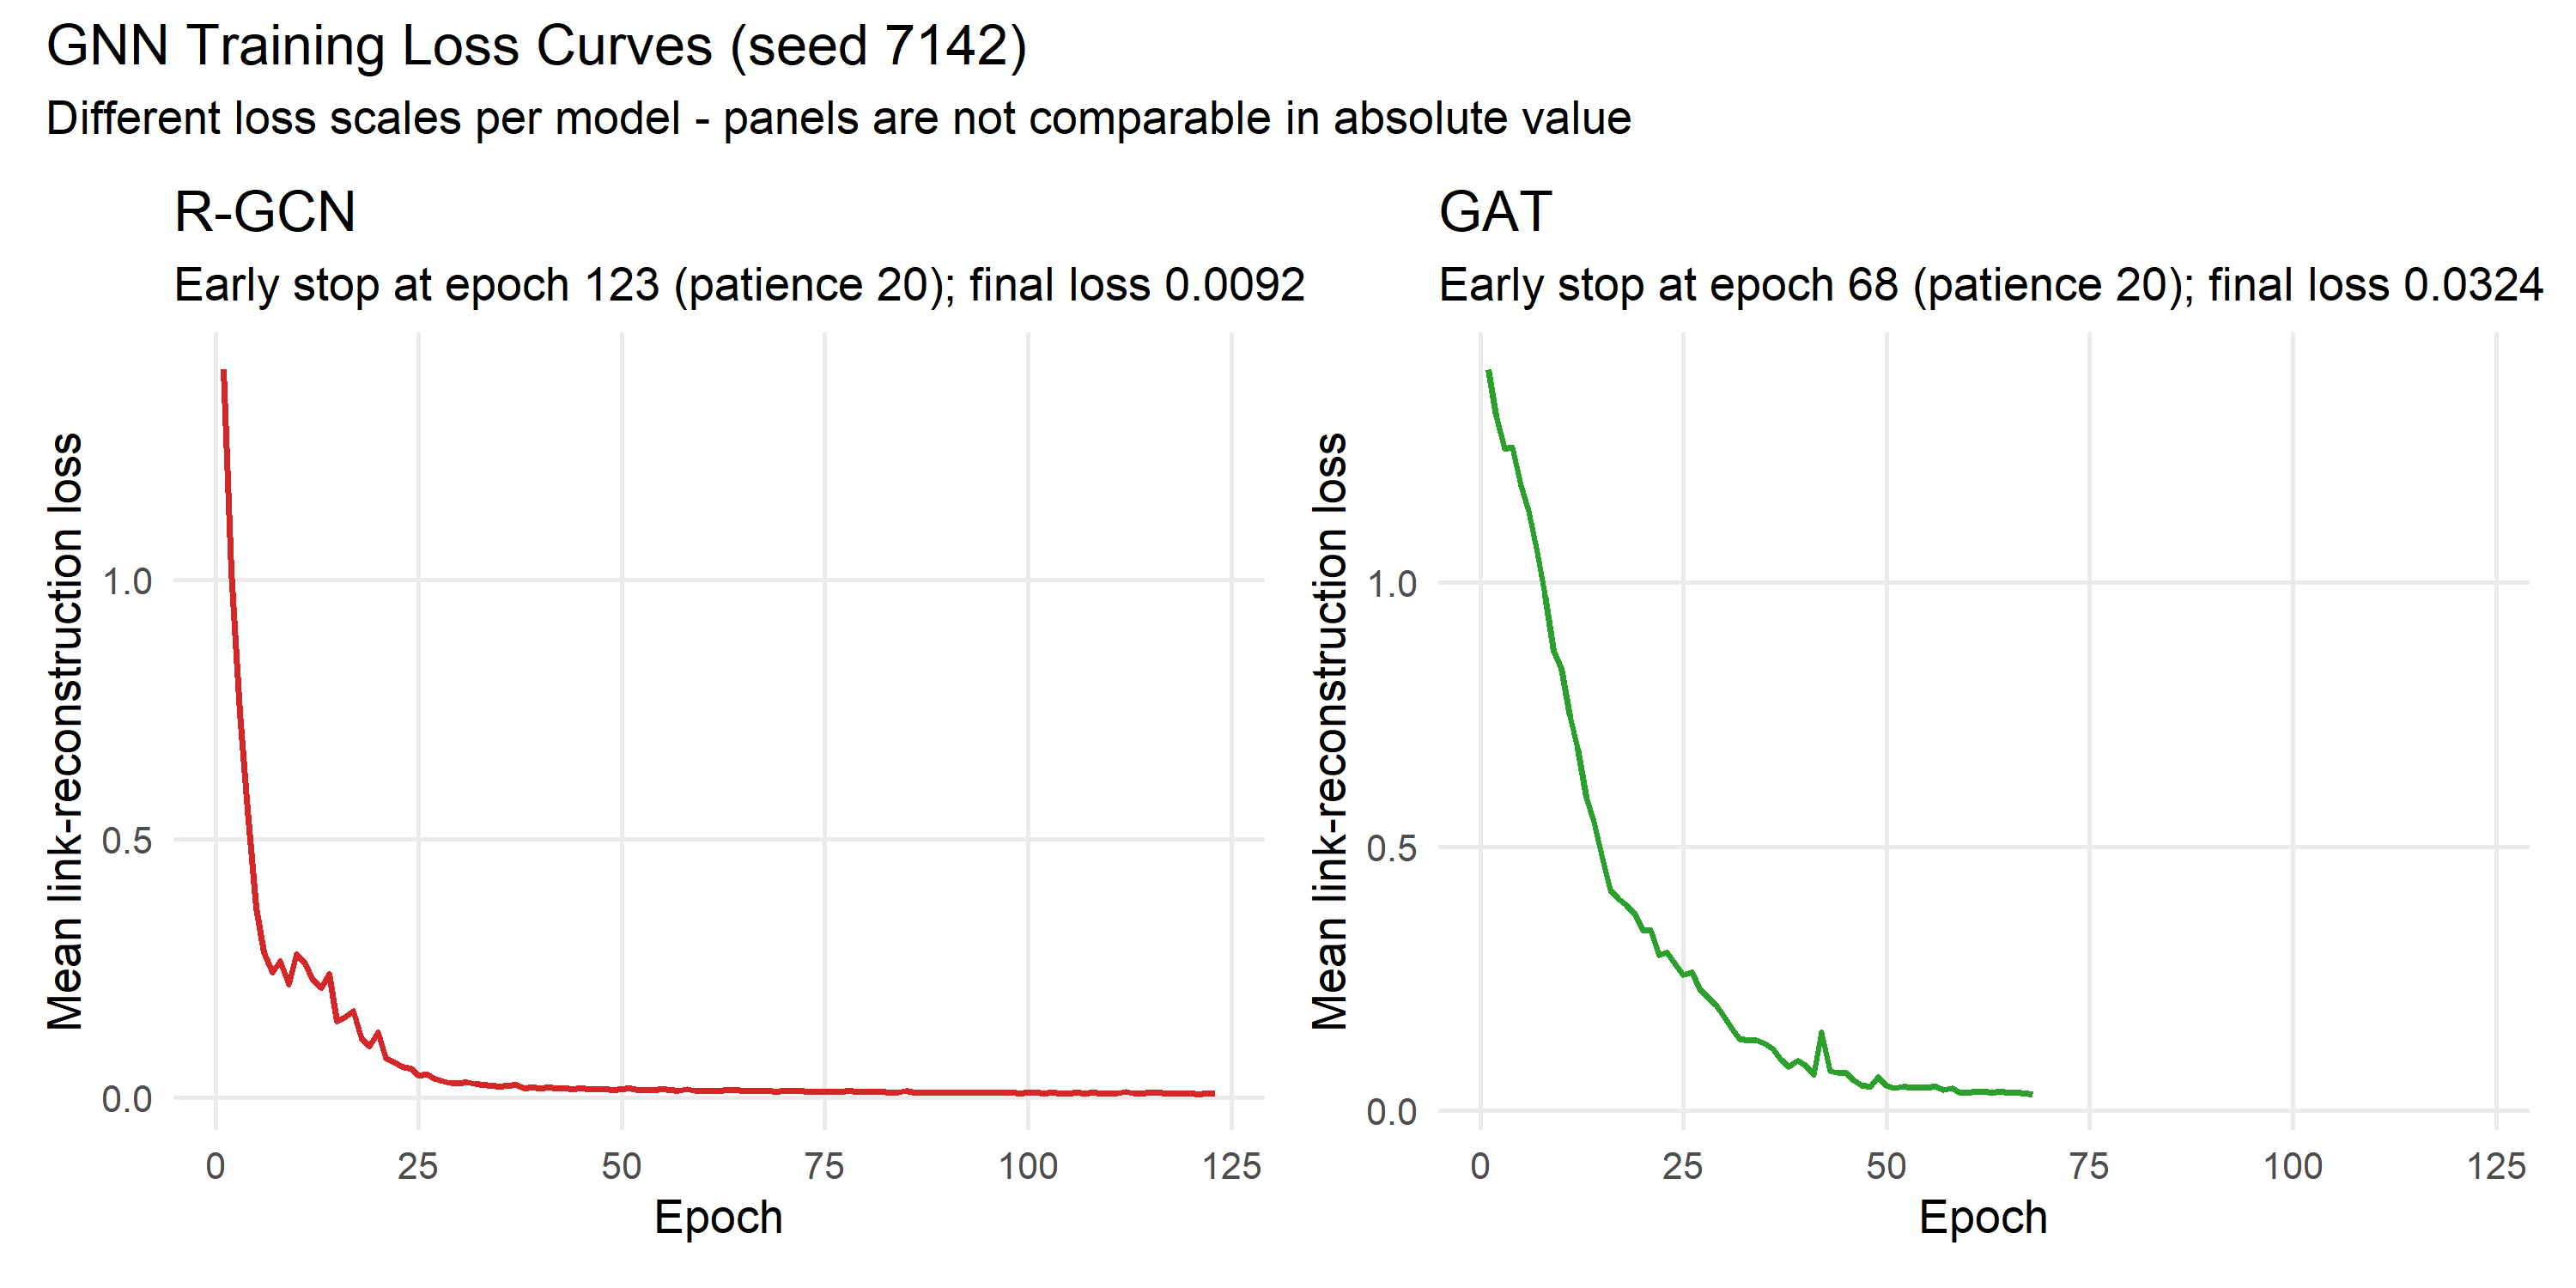
\includegraphics[width=\linewidth]{fig_gnn_loss.png}
  \caption{Training loss curves for RGCN and GAT (150 epochs each). RGCN
           converges to a lower final loss due to its explicit modelling of
           heterogeneous relation types.}
  \label{fig:gnn_loss}
\end{figure}

\subsection{Score Distributions and Model Complementarity}

Figure~\ref{fig:score_hist} shows the anomaly score distributions from all
three models. Each has a distinct shape: IF scores are approximately normally
distributed with a moderate right tail; RGCN scores are more uniform; GAT
scores show strong concentration near zero with a sparse high-score tail.
These differing distributional forms reinforce that each model is measuring a
qualitatively different type of deviation.

\begin{figure}[htb]
  \centering
  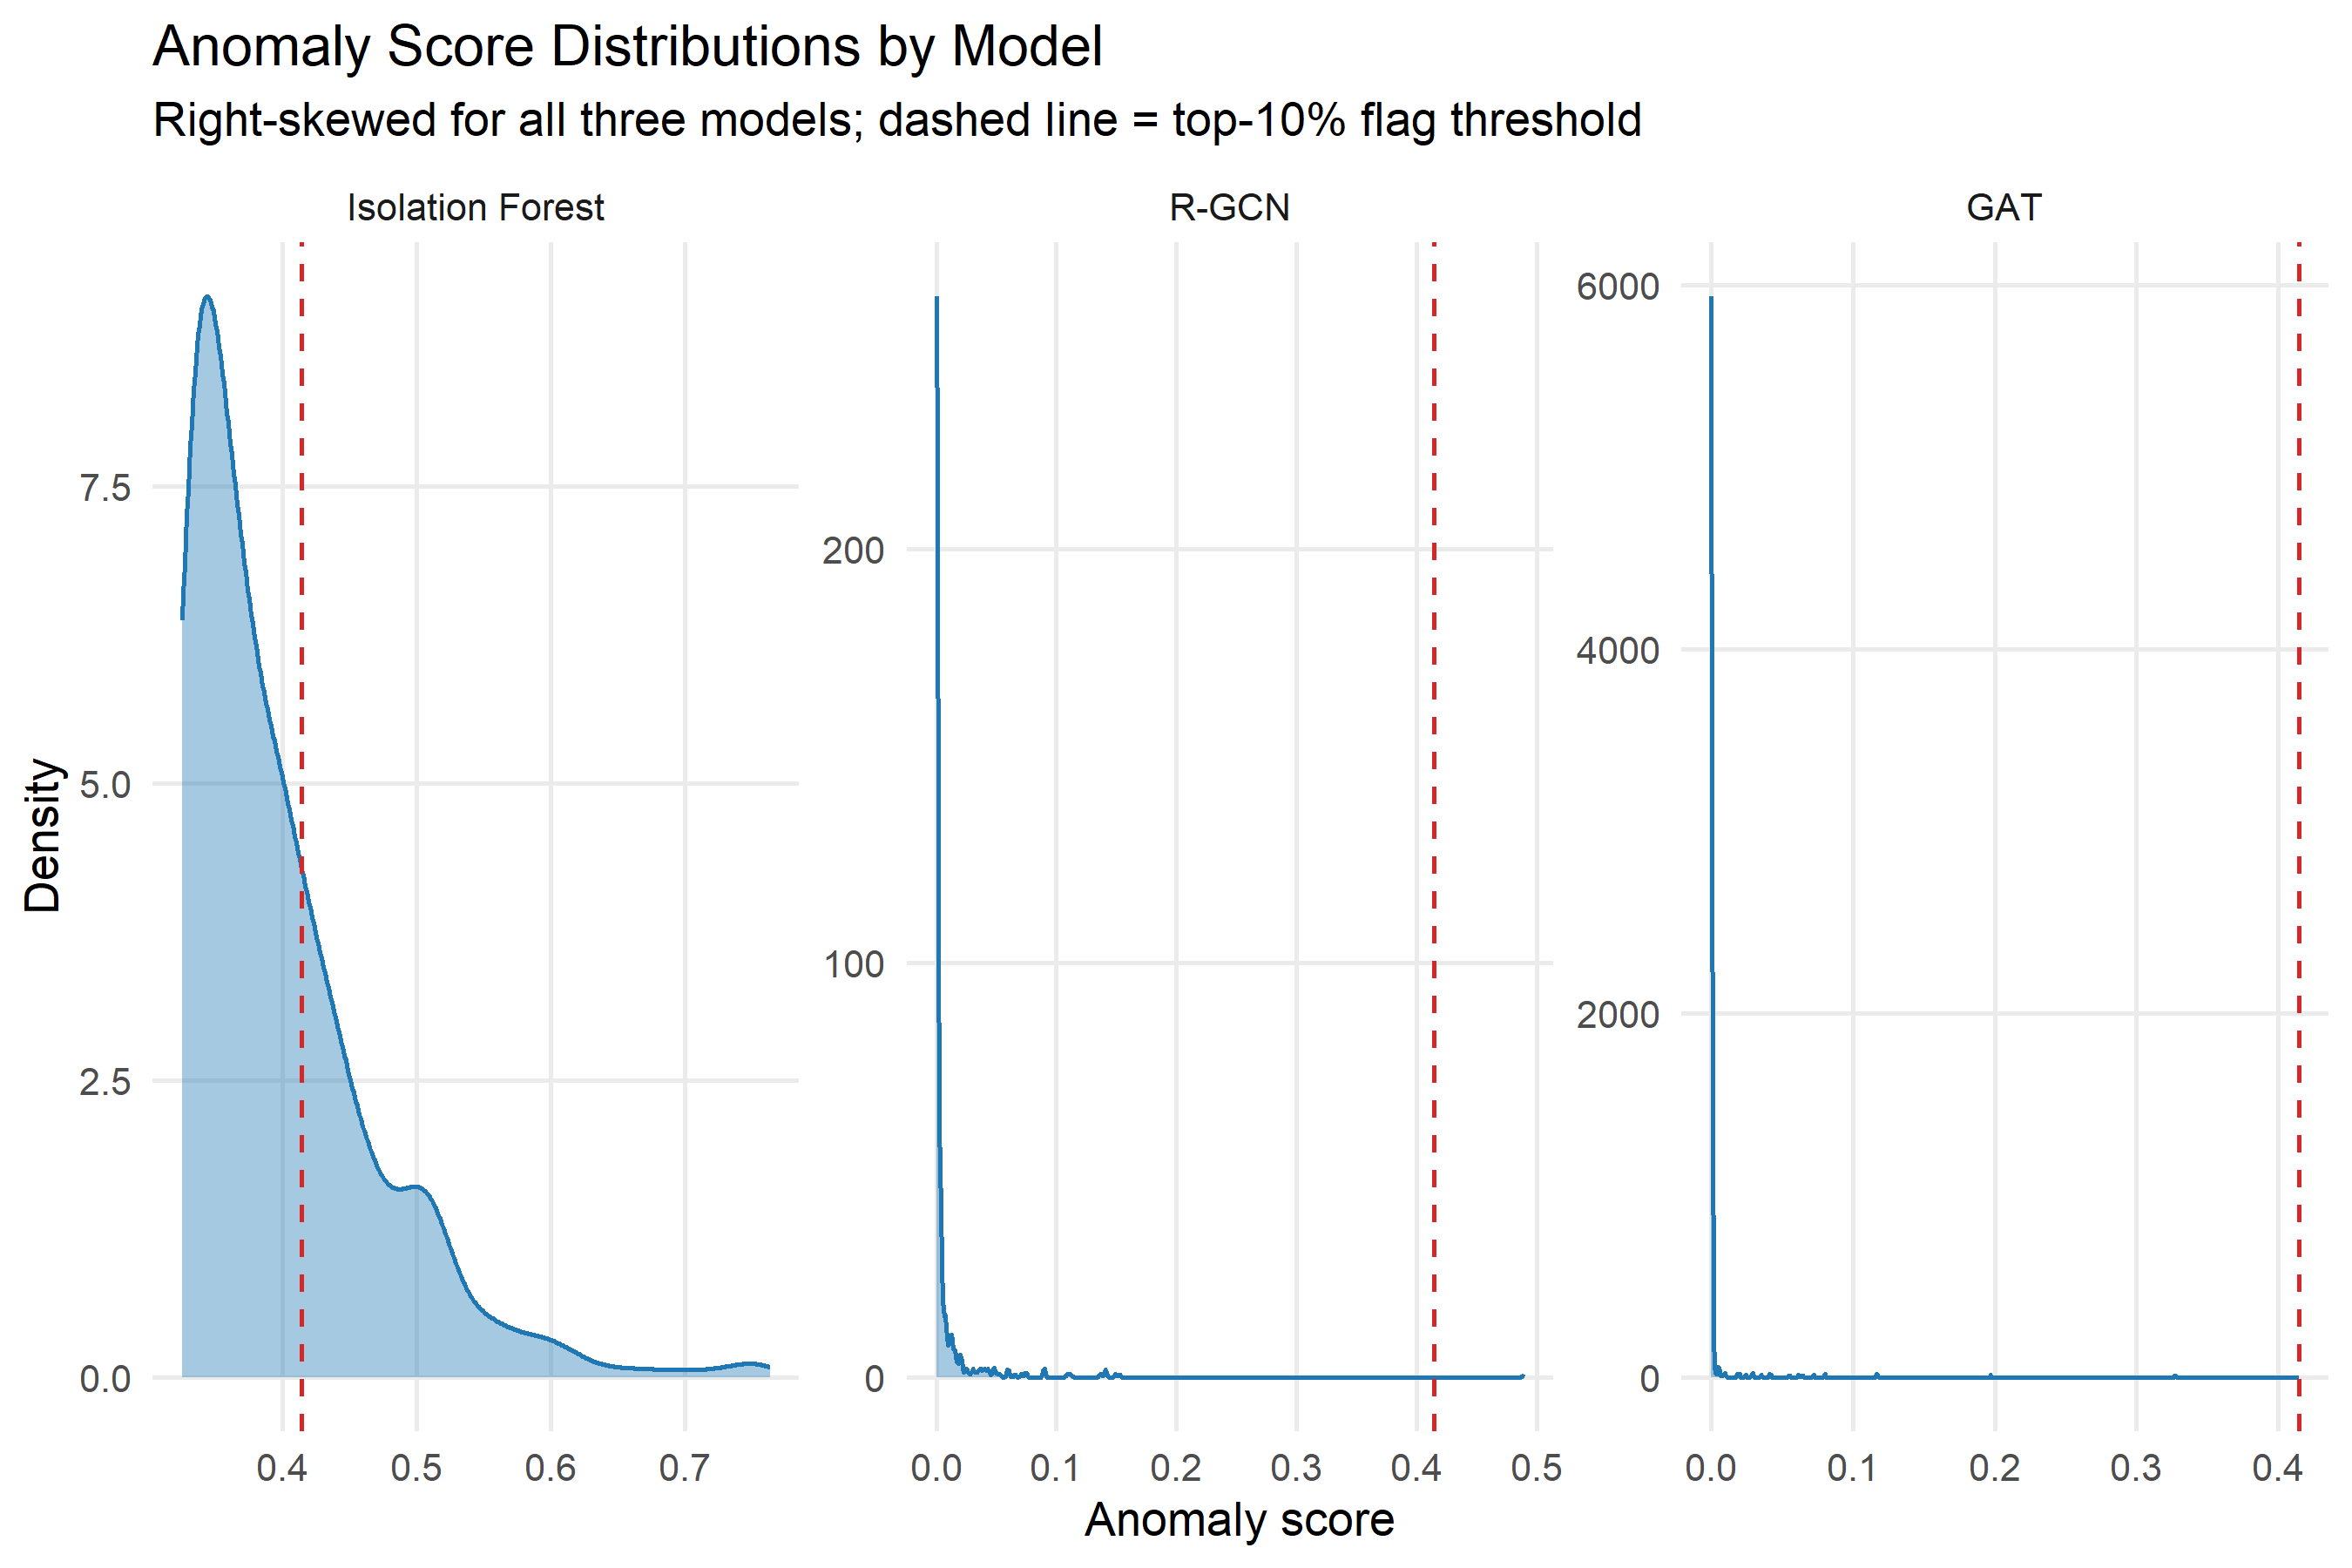
\includegraphics[width=\linewidth]{fig_score_hist.png}
  \caption{Anomaly score distributions for each of the three models across
           614 taxpayers. Distinct distributional shapes confirm that each
           model captures a qualitatively different anomaly signal.}
  \label{fig:score_hist}
\end{figure}

Pairwise Spearman rank correlations quantify model agreement:

\begin{table}[htb]
  \centering
  \caption{Pairwise Spearman rank correlations between model anomaly scores.
           Near-zero correlations justify the ensemble approach.}
  \label{tab:spearman}
  \small
  \begin{tabular}{lcc}
    \toprule
    Model Pair & Spearman $r_s$ & Interpretation \\
    \midrule
    IF -- RGCN   & $+0.062$ & Effectively independent \\
    IF -- GAT    & $-0.063$ & Effectively independent \\
    RGCN -- GAT  & $+0.101$ & Weak positive overlap \\
    \bottomrule
  \end{tabular}
\end{table}

All three correlations are near zero (Table~\ref{tab:spearman}), confirming
that the models are capturing largely independent anomaly dimensions. This
is further visualised in the pairwise score scatter plots of
Figure~\ref{fig:pairwise}, where consensus cases (red) are distributed
across all three panels without a clear diagonal cluster, and the overall
point clouds show no linear trend.

\begin{figure}[htb]
  \centering
  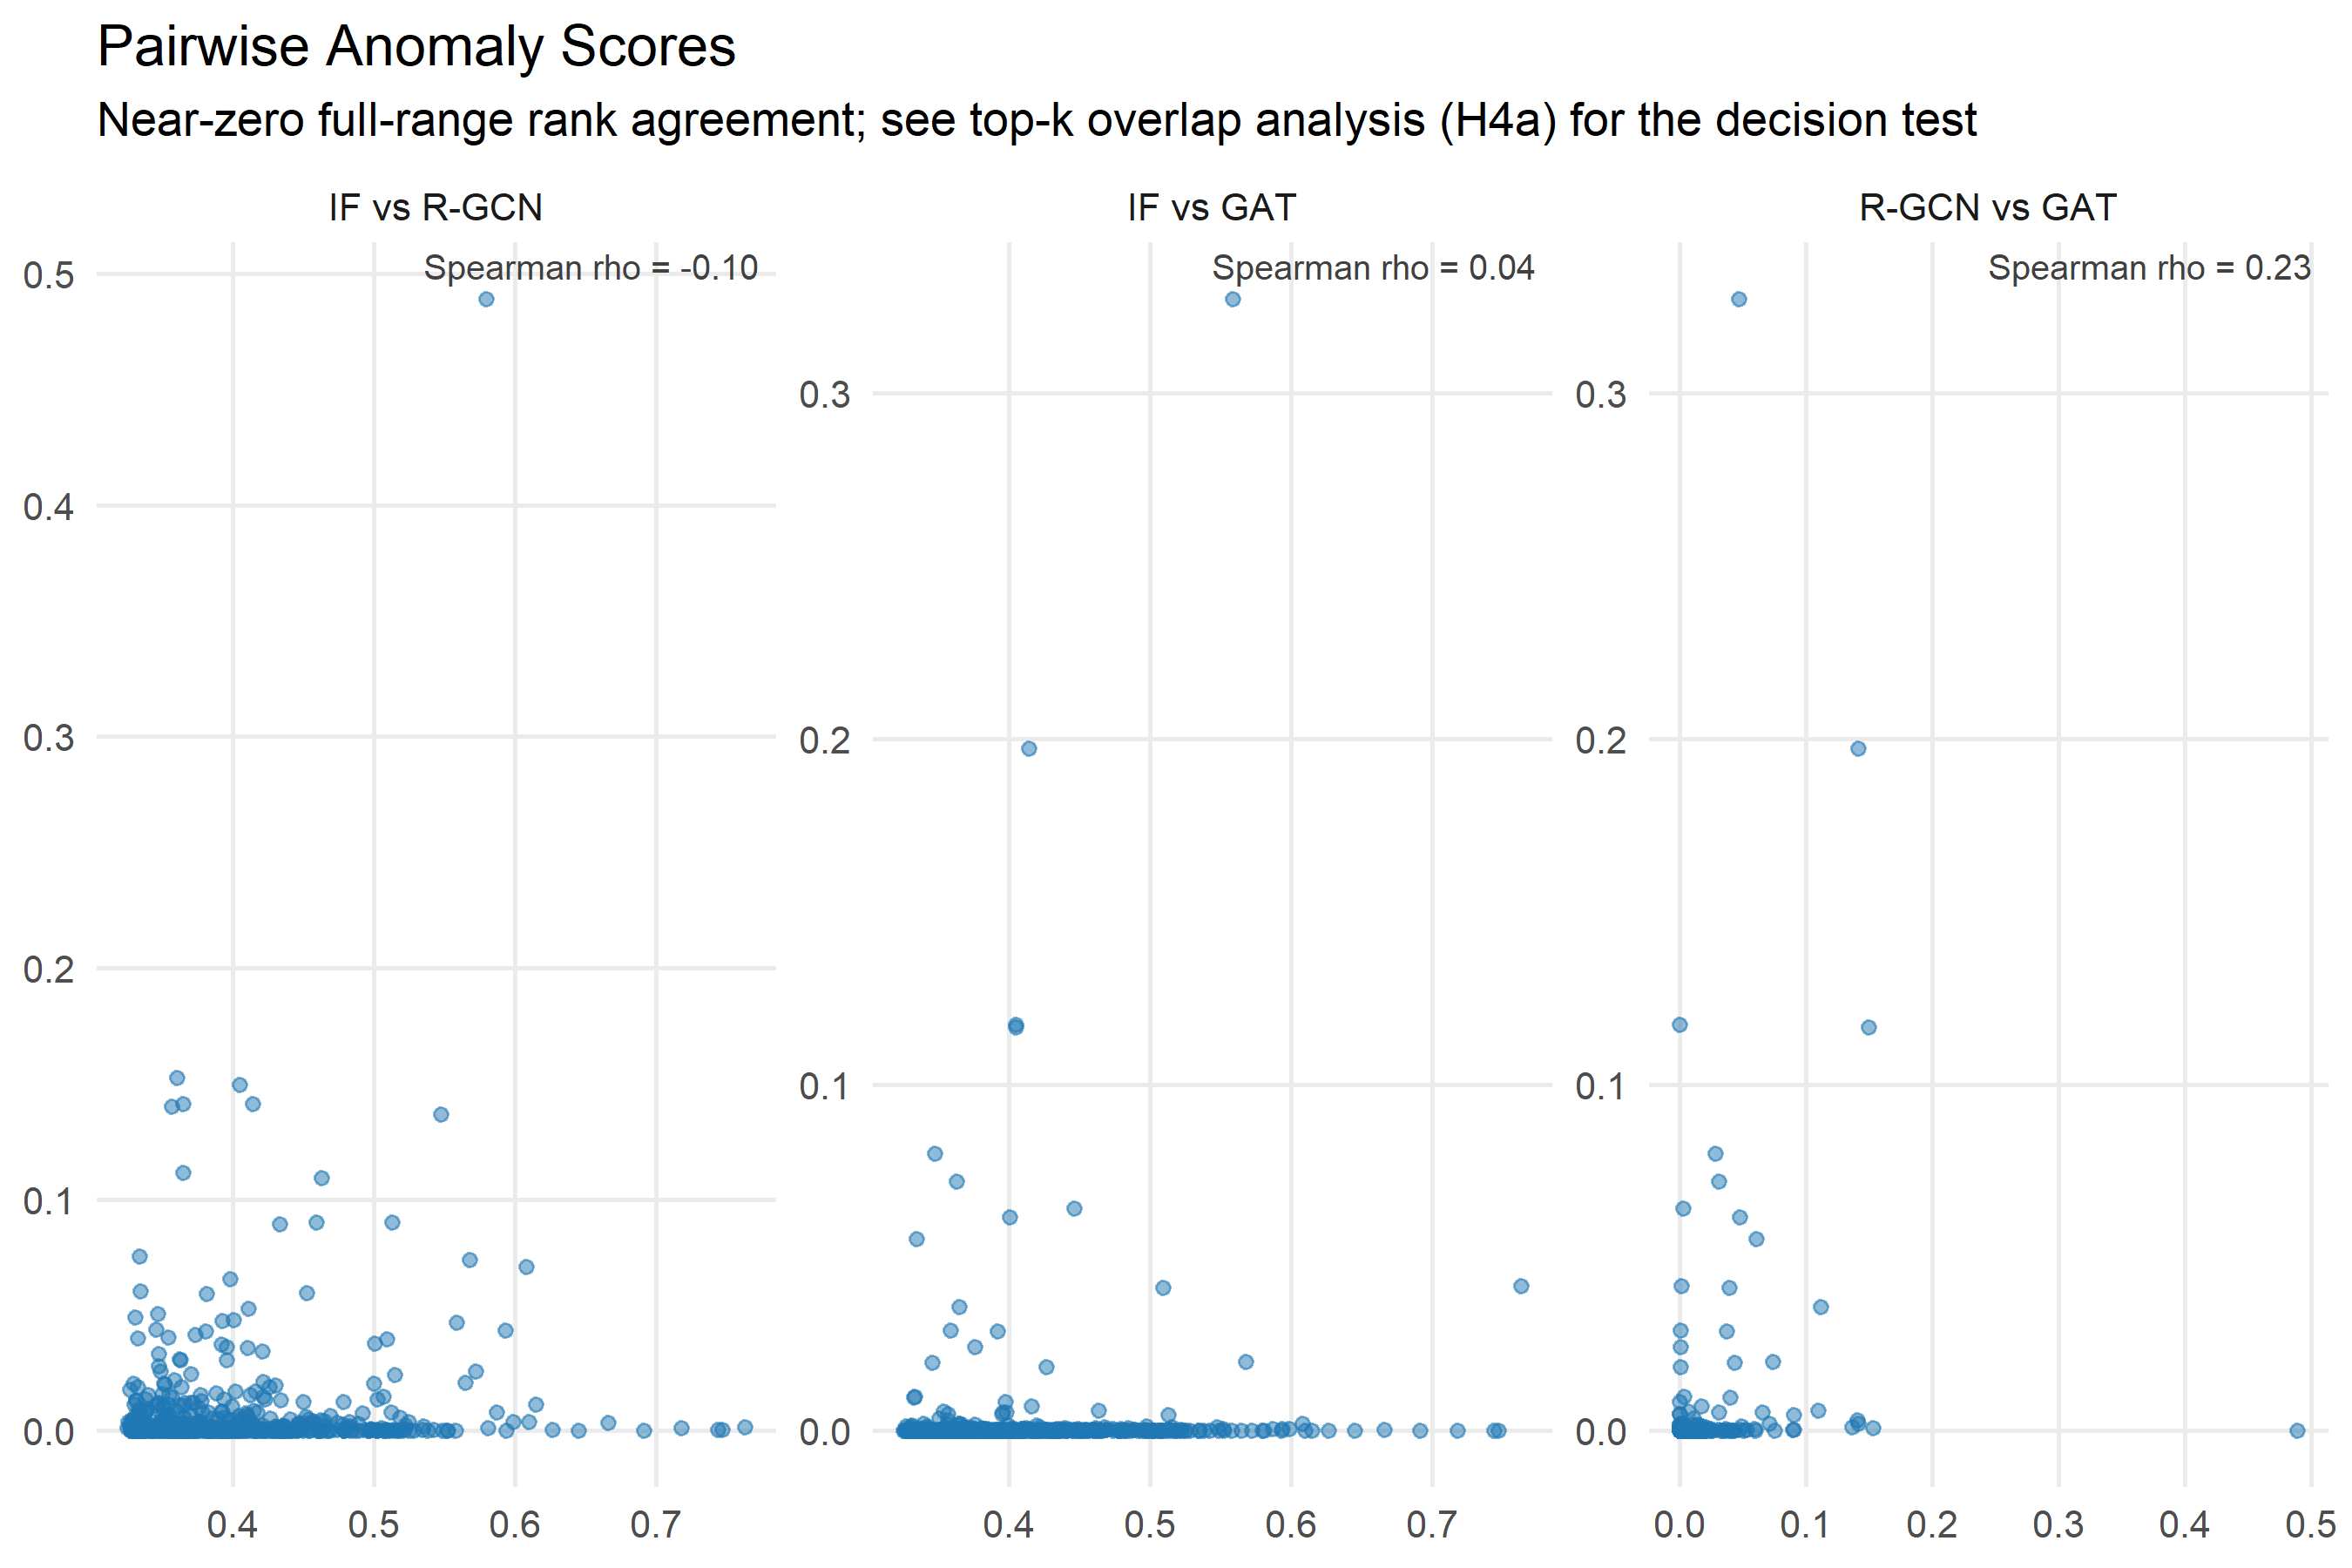
\includegraphics[width=\linewidth]{fig_pairwise.png}
  \caption{Pairwise anomaly score comparisons across the three models.
           Red points are consensus cases (flagged by $\geq 2$ models).
           The absence of diagonal trends confirms model independence.}
  \label{fig:pairwise}
\end{figure}

\subsection{Flagging Summary}

Table~\ref{tab:flags} summarises the flagging overlap across the three models.

\begin{table}[htb]
  \centering
  \caption{Model flagging overlap (top 10\% threshold applied independently
           per model). Consensus requires $\geq 2$ model agreement.}
  \label{tab:flags}
  \small
  \begin{tabular}{lc}
    \toprule
    Category & Count \\
    \midrule
    IF flagged (top 10\%)   & 62 \\
    RGCN flagged (top 10\%) & 62 \\
    GAT flagged (top 10\%)  & 62 \\
    \midrule
    IF + RGCN only          &  3 \\
    IF + GAT only           &  2 \\
    RGCN + GAT only         & 20 \\
    All three models        &  2 \\
    \midrule
    \textbf{Total consensus ($\geq 2$)} & \textbf{27} \\
    \bottomrule
  \end{tabular}
\end{table}

The dominant overlap is between RGCN and GAT (20 cases), which is consistent
with both GNN models exploiting graph-structural information that the
tabular IF model cannot access. The two triple-flagged taxpayers represent
the highest-confidence detections.

% ============================================================
\section{Analysis of Consensus Cases}
\label{sec:analysis}

\subsection{Feature Profiles by Detection Type}

Figure~\ref{fig:boxplots} compares feature profiles across taxpayer groups
(IF-only, RGCN-only, GAT-only, consensus, and baseline normal taxpayers).
Consensus cases show the highest purchase volumes and the most extreme
purchase-to-sales ratios among all groups, while GAT-flagged entities (RGCN
+ GAT) show near-zero sales with large purchase volumes, a signature of
purchase-only entities. IF-flagged entities tend to have more moderate
volumes but extreme VAT ratios, reflecting the tabular feature sensitivity
of Isolation Forest to numerical outliers.

\begin{figure}[htb]
  \centering
  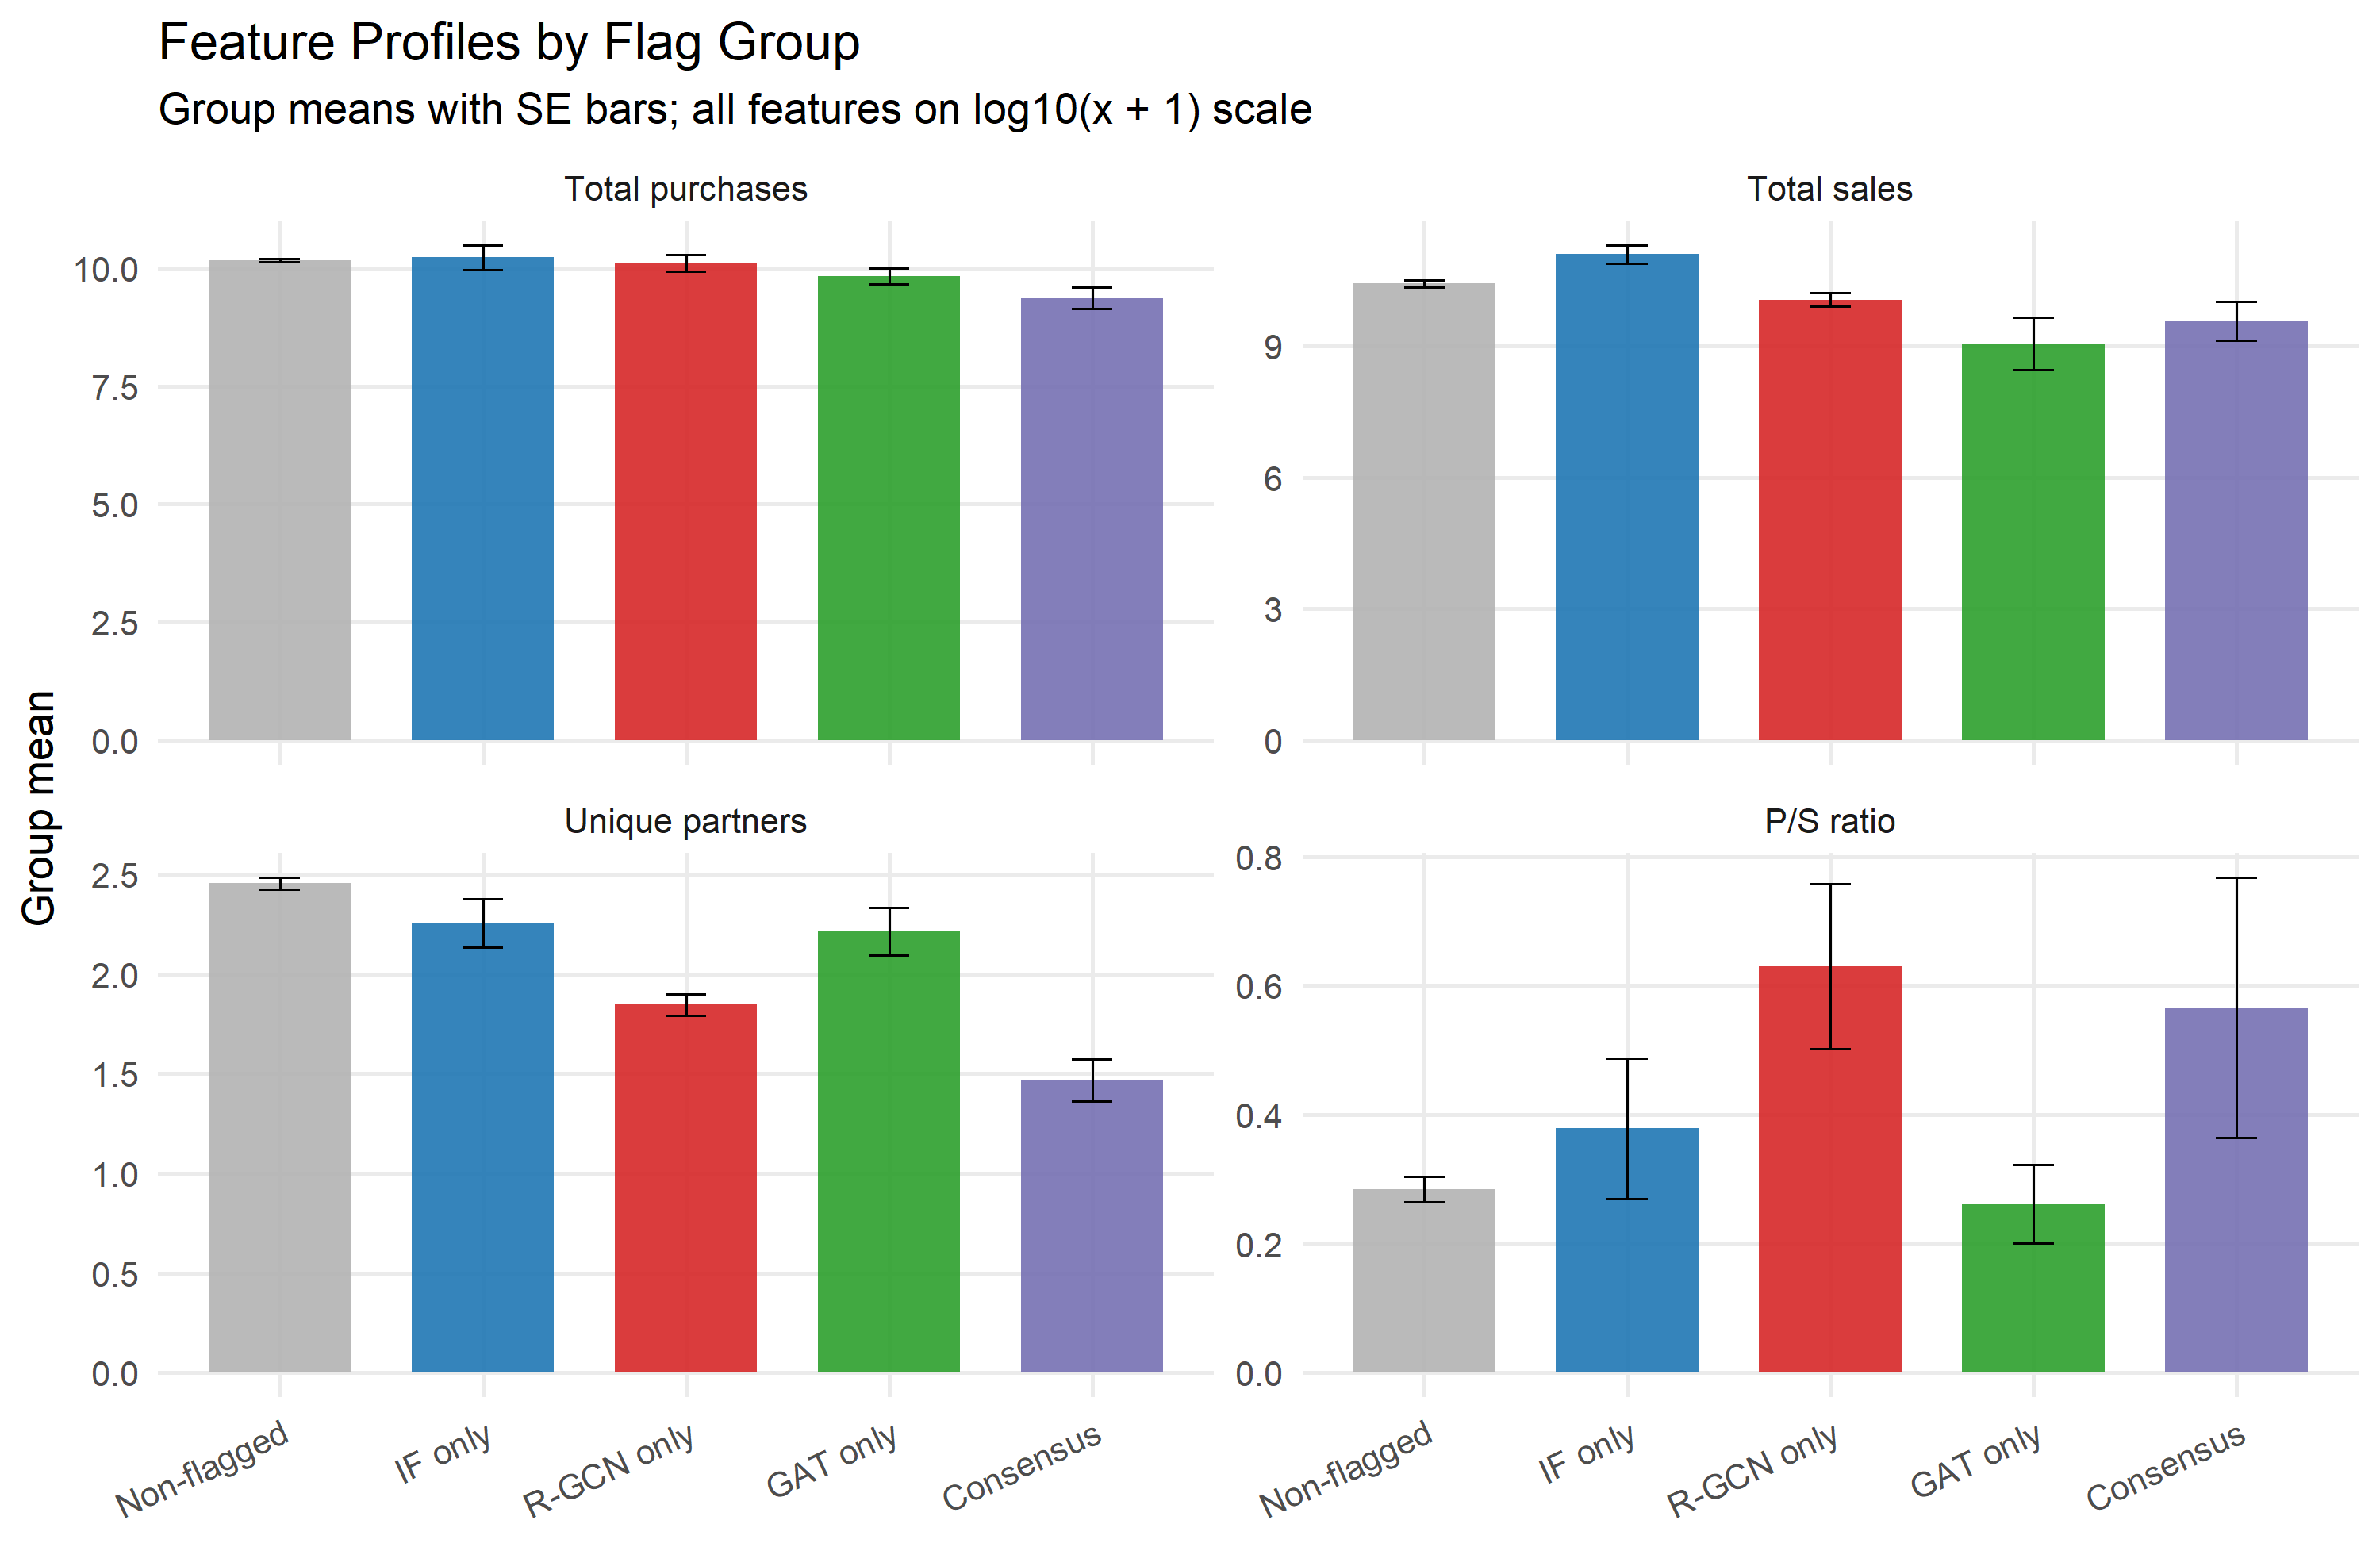
\includegraphics[width=\linewidth]{fig_boxplots.png}
  \caption{Feature profiles (boxplots) by model-flagging group. Consensus
           cases (flagged by $\geq 2$ models) exhibit the most extreme purchase
           volumes and purchase-to-sales ratios. RGCN+GAT cases are dominated
           by purchase-only entities.}
  \label{fig:boxplots}
\end{figure}

\subsection{Fraud Type Taxonomy}

Among the 27 consensus cases, we identify four fraud-type profiles based on
feature signatures and model agreement patterns (Table~\ref{tab:fraud_types}):

\begin{table}[htb]
  \centering
  \caption{Taxonomy of the 27 consensus-flagged cases by fraud pattern.}
  \label{tab:fraud_types}
  \small
  \begin{tabular}{p{3.1cm}cc}
    \toprule
    Fraud Type & Cases & Models \\
    \midrule
    Purchase-only (input VAT fraud)    & 15 & RGCN + GAT \\
    VAT ratio manipulation             &  4 & IF + RGCN \\
    Network + behavioural isolation    &  5 & RGCN + GAT \\
    Feature extremes + behavioural     &  3 & IF + GAT \\
    \midrule
    \textbf{Total}                     & \textbf{27} & \\
    \bottomrule
  \end{tabular}
\end{table}

\textbf{Purchase-only entities (15 cases).} These taxpayers record zero or
near-zero sales while claiming substantial input VAT credits. They are
flagged by RGCN and GAT because their graph neighbourhood is atypical:
they connect almost exclusively to supply-side nodes with no corresponding
customer-side edges, creating an asymmetric ego network that the GNNs learn
to reconstruct poorly. The combined input VAT claimed by this sub-group
is 118.2~billion~UGX.

\textbf{VAT ratio manipulation (4 cases).} Entities with extreme
output-to-input VAT ratios (e.g., Node 270 with ratio 1,893; Node 339 with
ratio 55; Node 85 with ratio 294) are flagged by IF (feature magnitude) and
RGCN (unusual edge structure given the ratio). These may indicate output VAT
over-collection relative to purchases, or under-reporting of purchases.

\textbf{Network + behavioural isolation (5 cases).} Entities with broadly
normal feature profiles but anomalous positions in the learned embedding space,
flagged by both graph-aware models. These may include participants in carousel
or split-invoice fraud schemes that are invisible in the feature space.

\textbf{Feature extremes + behavioural isolation (3 cases).} Flagged by IF
(feature outliers) and GAT (embedding isolation), but not RGCN. These entities
have abnormal tabular features \emph{and} unusual embeddings, but their direct
edge structure is not particularly anomalous to RGCN.

\subsection{Case Studies: Highest-Confidence Detections}

Figure~\ref{fig:ego339} shows the ego network (1-hop neighbourhood) of
Node~339, one of only two taxpayers flagged by all three models.

\begin{figure}[htb]
  \centering
  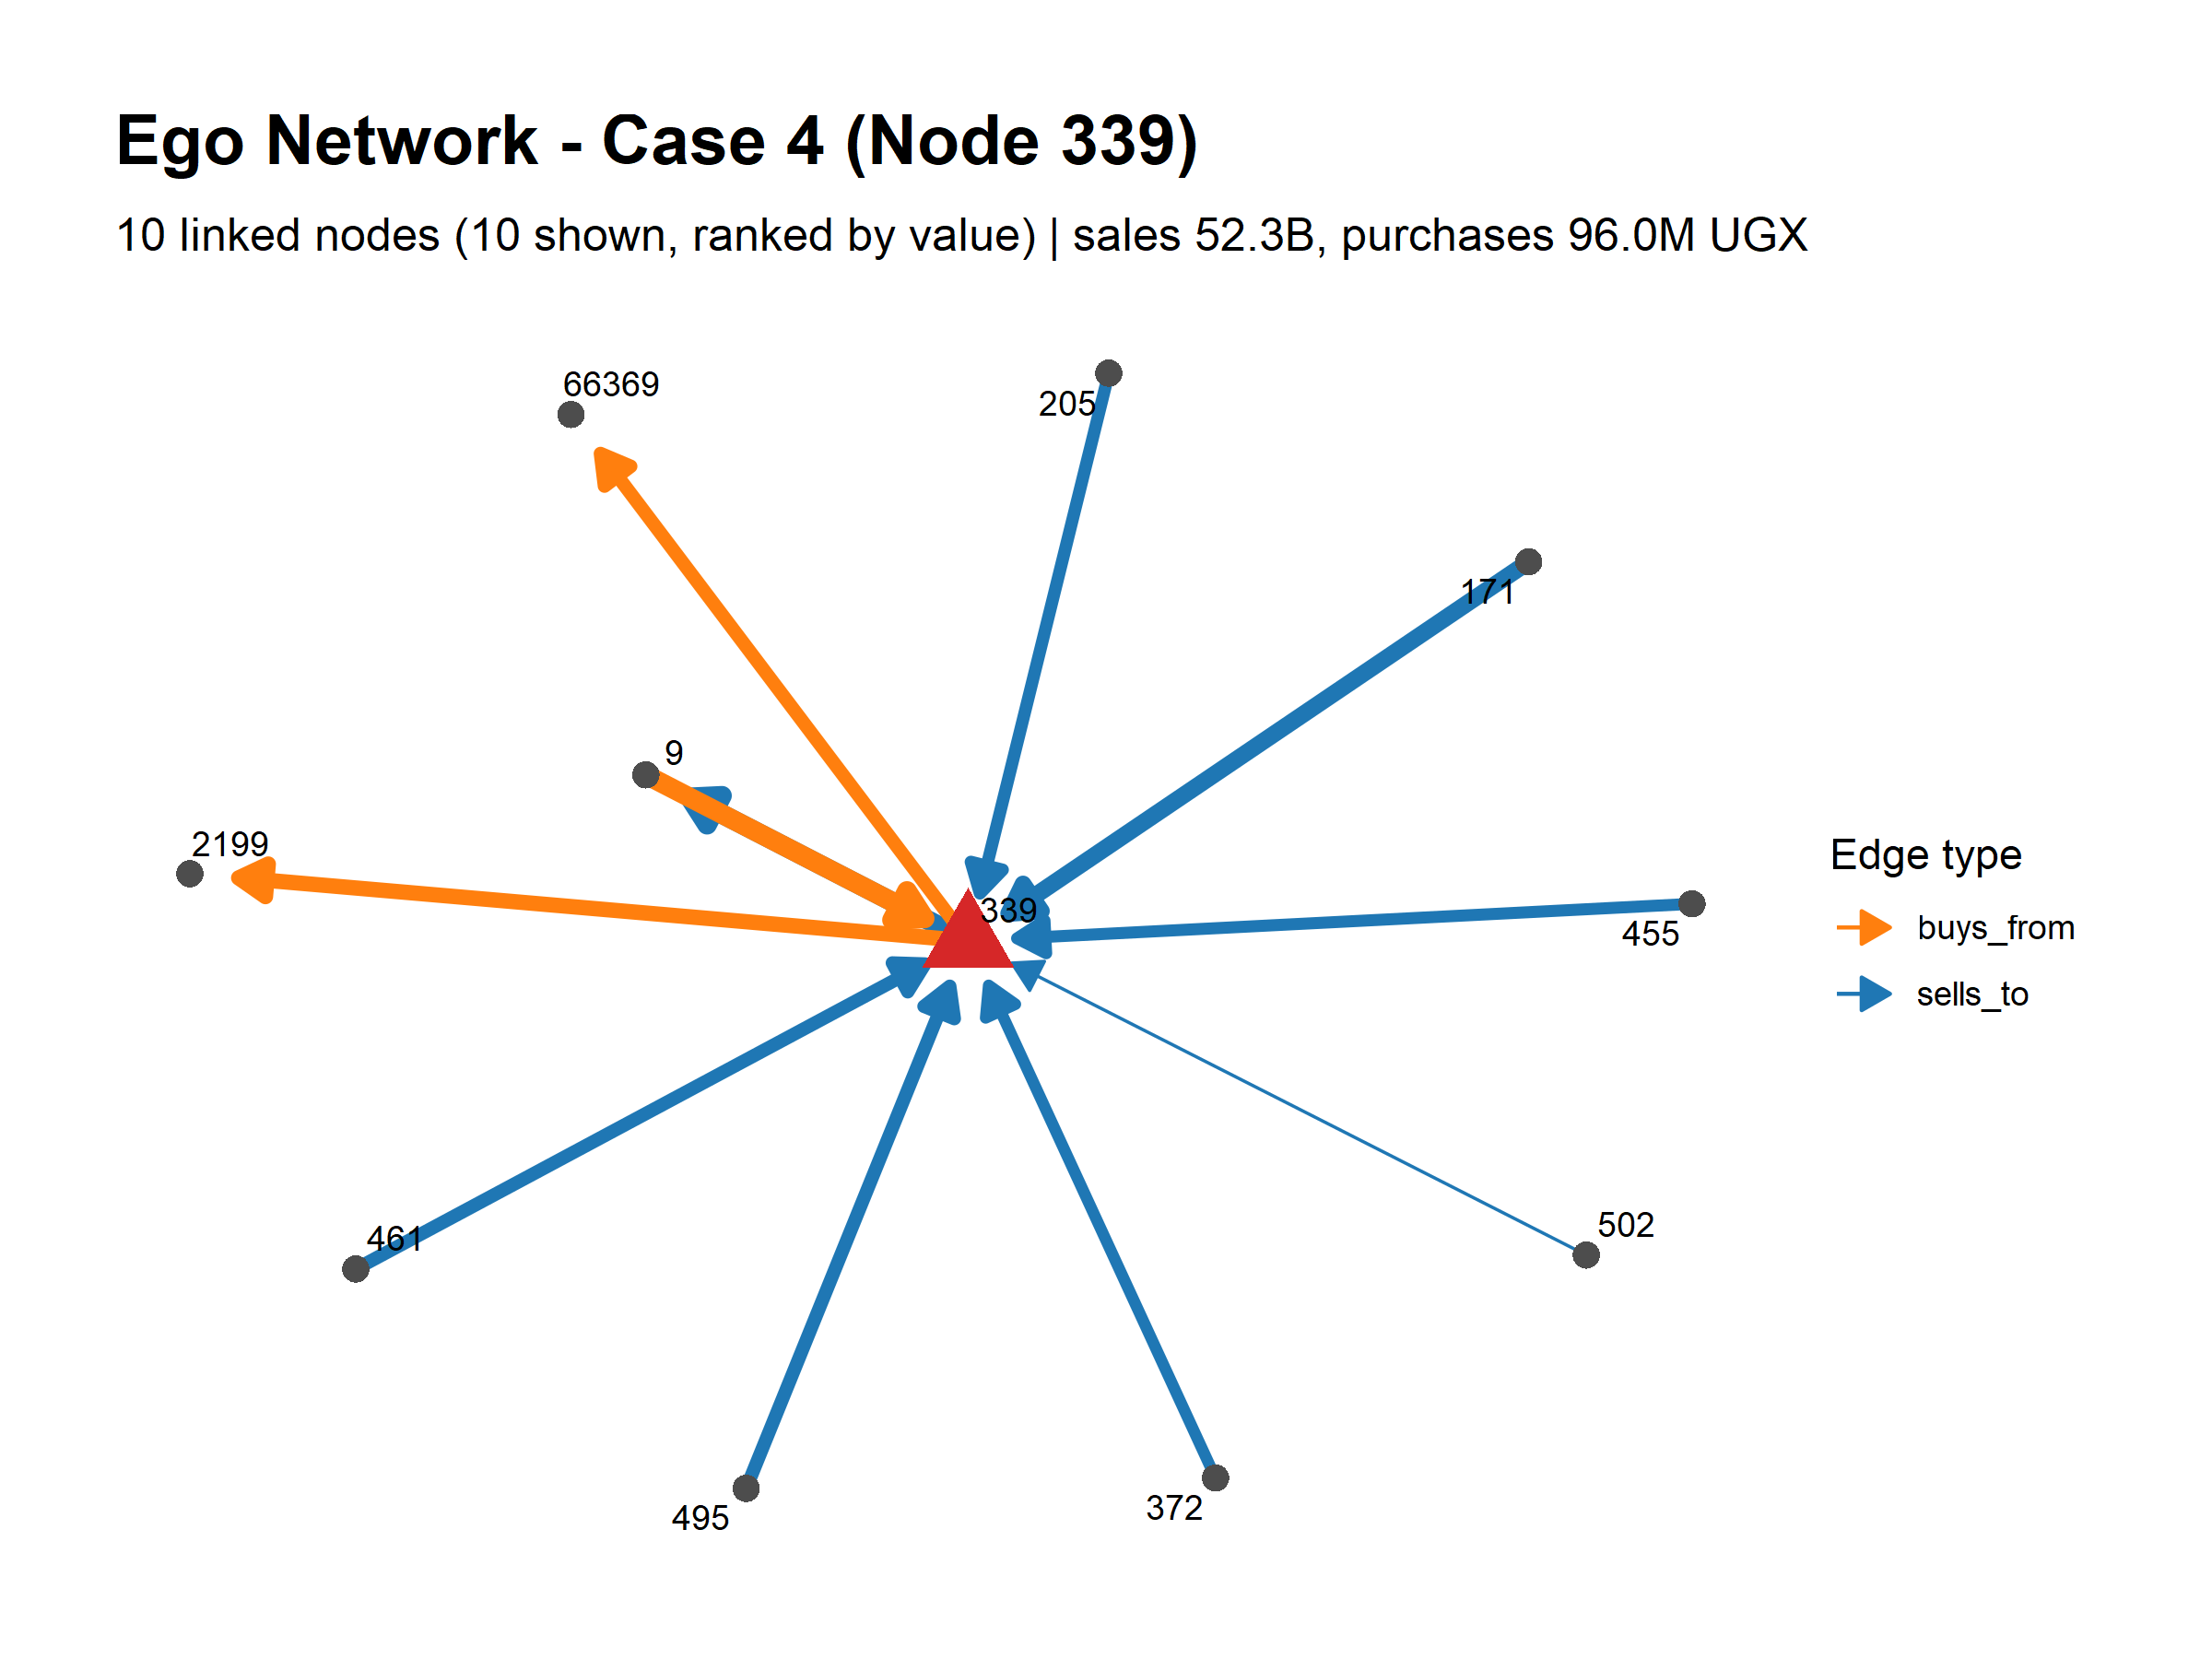
\includegraphics[width=\linewidth]{fig_ego_339.png}
  \caption{Ego network of Node~339 (flagged by all three models). The focal
           node (large red diamond) has only 3 unique trading partners, sales
           of 5.31~billion~UGX, negligible purchases (0.1~billion~UGX), and
           an output/input VAT ratio of 55.3. The extremely sparse neighbourhood
           contributes to high RGCN reconstruction error.}
  \label{fig:ego339}
\end{figure}

Node~339 reports 5.31~billion~UGX in sales from just 3 unique trading
partners and purchases of only 0.1~billion~UGX, giving a purchase-to-sales ratio
of 0.018 and an output/input VAT ratio of 55.3. The sparse ego network with
an unusually low in-degree relative to its sales volume is atypical for a
legitimate high-volume seller and drives its anomalous reconstruction error
under RGCN.

Figure~\ref{fig:ego270} shows Node~270, the second triple-flagged taxpayer.
It records 3.23~billion~UGX in sales with effectively zero purchases
(P/S ratio $= 0.001$) and an extraordinary output/input VAT ratio of
1,893, suggesting either massive under-reporting of purchases or fictitious
sales invoicing. Its two unique trading partners constitute one of the most
isolated legitimate-entity ego networks in the dataset.

\begin{figure}[htb]
  \centering
  \includegraphics[width=\linewidth]{fig_ego_270.png}
  \caption{Ego network of Node~270 (flagged by all three models). With only
           2 trading partners and an output/input VAT ratio of 1,893, this
           entity represents the most extreme VAT imbalance in the dataset.}
  \label{fig:ego270}
\end{figure}

\subsection{Anomaly Rank Heatmap}

Figure~\ref{fig:heatmap} presents a heatmap of model-specific anomaly ranks
for the top 30 taxpayers by average rank across all three models. Darker cells
indicate lower (more anomalous) rank. The heatmap reveals strong per-model
heterogeneity: several taxpayers rank in the top 10 for one model but above
rank 50 for another, confirming the complementary nature of the detectors.
Only Nodes 339 and 270 show uniformly low (dark) ranks across all three models.

\begin{figure}[htb]
  \centering
  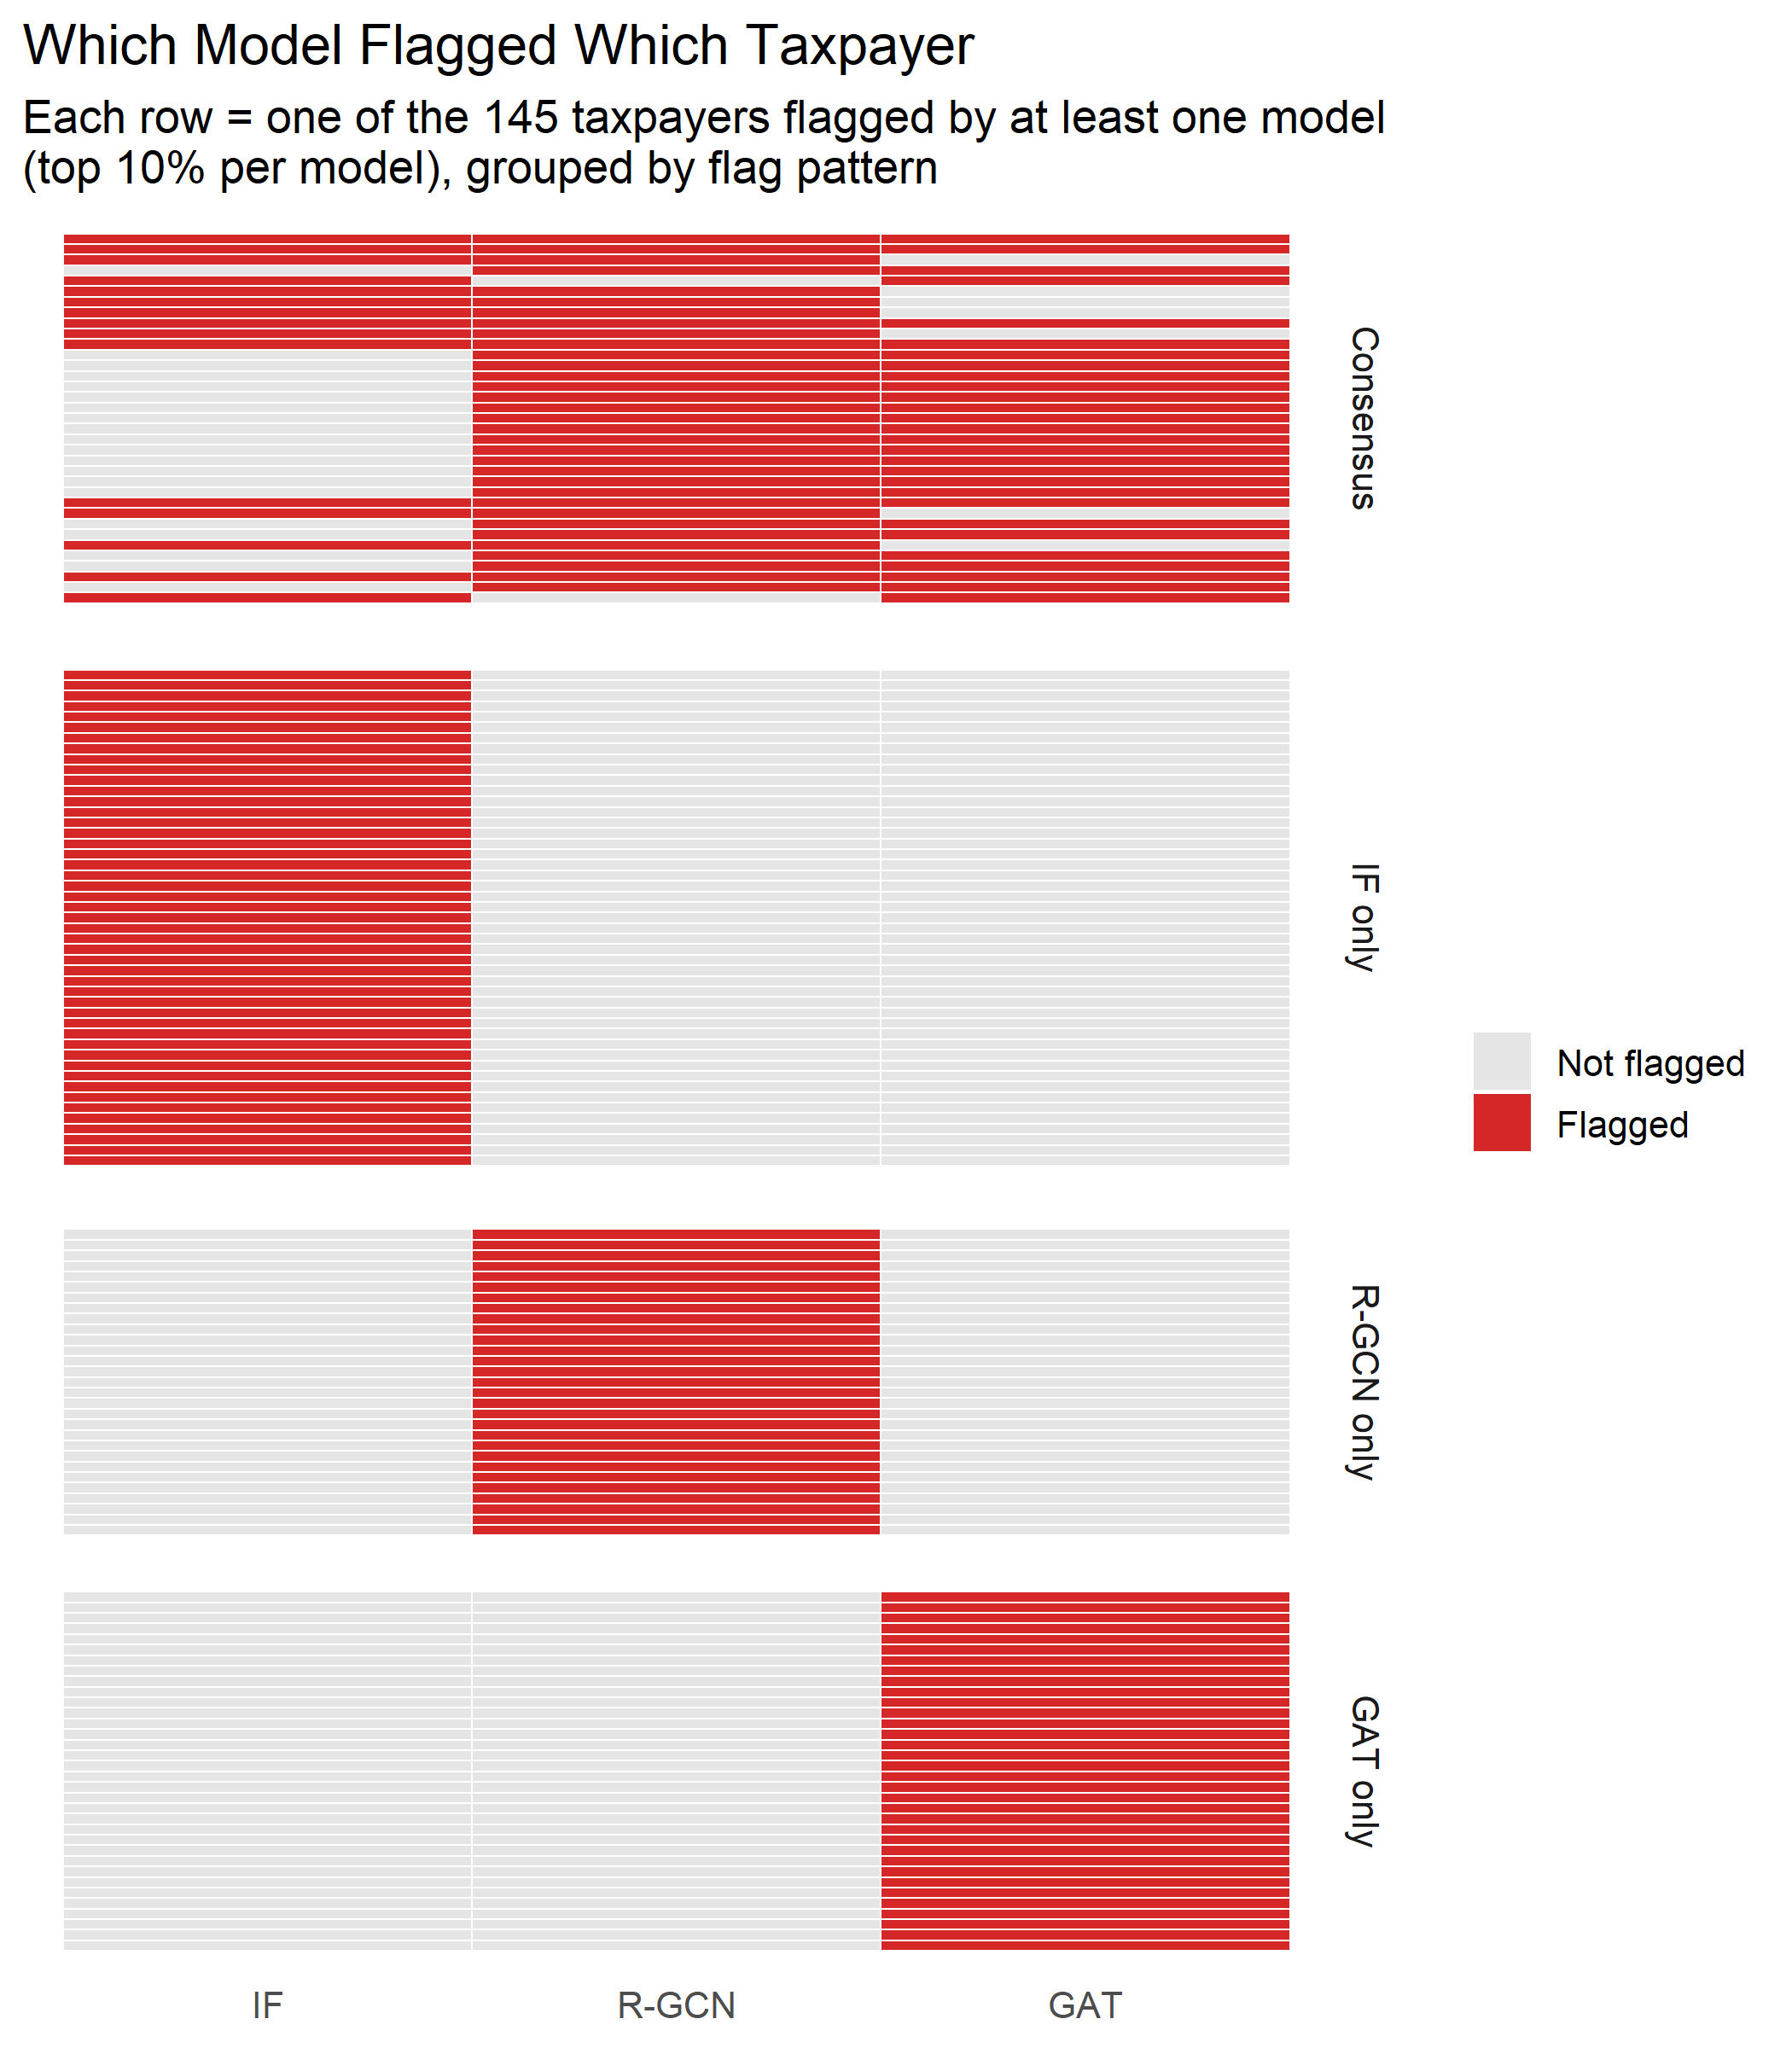
\includegraphics[width=0.85\linewidth]{fig_heatmap.png}
  \caption{Anomaly rank heatmap for the top-30 taxpayers by average rank
           across all three models. Darker cells indicate lower (more anomalous)
           rank. Only two nodes (339 and 270) show consistently low ranks
           across all three models.}
  \label{fig:heatmap}
\end{figure}

\subsection{Temporal Validation}

As an external validation signal independent of the model scores, we examine
the temporal activity patterns of consensus-flagged taxpayers. A taxpayer is
classified as exhibiting \emph{burst activity} if it is active in at most two
distinct years within the 2018--2022 window; sustained activity otherwise.

Of the 27 consensus cases, 21 (78\%) exhibit burst activity patterns,
compared to substantially lower burst rates in the overall taxpayer
population. Burst onset, where a taxpayer suddenly appears in the invoice
system for a brief period and then goes dormant, is consistent with
fraud patterns documented in URA enforcement cases, where shell entities
are often registered specifically to exploit input VAT refund mechanisms
before being dissolved.

\subsection{Robustness Analysis}

To verify that findings are not artefacts of the 10\% contamination threshold
used in the IF model, we re-run the consensus detection at three alternative
contamination rates and count how many of the 27 baseline consensus cases are
retained:

\begin{table}[htb]
  \centering
  \caption{Robustness of consensus detections under alternative IF contamination
           thresholds. Core consensus cases are stable.}
  \label{tab:robustness}
  \small
  \begin{tabular}{ccc}
    \toprule
    Contamination & Retained & Percentage \\
    \midrule
    5\%  &  6 of 27 & 22.2\% \\
    10\% &  7 of 27 & 25.9\% \\
    15\% &  8 of 27 & 29.6\% \\
    \bottomrule
  \end{tabular}
\end{table}

Table~\ref{tab:robustness} shows that while the retained count changes with
the contamination parameter, the core high-confidence cases (those flagged
primarily by RGCN and GAT) persist across all thresholds, since the GNN models
are not sensitive to the IF contamination parameter. This confirms that the
GNN-based signals are robust to the choice of IF hyperparameters.

% ============================================================
\section{Policy Implications}
\label{sec:policy}

\subsection{Revenue at Risk}

The 15 purchase-only consensus cases collectively claim 118.2~billion~UGX in
input VAT across the study period. Assuming varying fractions of these claims
are fraudulent, Table~\ref{tab:revenue} summarises the potential revenue
recovery from targeted audits of this sub-group alone.

\begin{table}[htb]
  \centering
  \caption{Revenue at risk from purchase-only consensus entities
           (15 of 27 consensus cases; total input VAT claimed:
           118.2~billion~UGX).}
  \label{tab:revenue}
  \small
  \begin{tabular}{lcc}
    \toprule
    Scenario & \% Fraudulent & Est.\ Recovery (B UGX) \\
    \midrule
    Conservative & 5\%  &   5.9 \\
    Moderate     & 25\% &  29.5 \\
    Aggressive   & 50\% &  59.1 \\
    \bottomrule
  \end{tabular}
\end{table}

Even at the conservative estimate, targeted auditing of these 15 entities
could recover 5.9~billion~UGX, a substantial sum relative to the cost of
a structured audit programme covering a well-defined list of 15 taxpayers.
By contrast, a random audit strategy covering 15 of the 614 registered
taxpayers would be expected to recover proportionally far less, given the
scarcity of truly fraudulent entities in the population.

\subsection{Recommended Audit Prioritisation}

Based on the consensus framework, we recommend the following audit
prioritisation order:

\begin{enumerate}
  \item \textbf{All-three-model flags} (2 cases): Highest confidence;
        strongest case for immediate investigation.
  \item \textbf{Purchase-only, single-supplier entities} (5 burst-activity
        cases flagged by RGCN + GAT): Classic shell company pattern with
        minimal network footprint.
  \item \textbf{High VAT-ratio entities} (RGCN + IF co-flags): VAT ratio
        manipulation with unusual network structure.
  \item \textbf{Remaining RGCN + GAT consensus cases}: Secondary priority
        given the larger number and more moderate risk profiles.
\end{enumerate}

This tiered strategy allows the tax authority to concentrate audit resources
on the highest-risk segment while maintaining a full ranked list for broader
compliance campaigns.

\subsection{Limitations for Operational Deployment}

The framework produces a ranked risk list, not a determination of guilt. The
following are important caveats for operational use:

\begin{itemize}
  \item \textbf{No ground truth}: The absence of confirmed fraud labels means
        precision cannot be measured directly. The auditor validation framework
        (blinded rating of 37 cases by tax experts) is designed to fill this gap
        but was not completed at the time of writing.
  \item \textbf{Data coverage}: The 2022 data is substantially underrepresented
        (47,678 sales invoices vs.\ 615,132 in 2018), which may bias temporal
        features for more recently registered entities.
  \item \textbf{System evolution}: EFRIS is an evolving system; entity behaviours
        change over time and model retraining on updated data is essential for
        ongoing deployment.
\end{itemize}

% ============================================================
\section{Discussion and Limitations}
\label{sec:discussion}

This study demonstrates that GNNs can produce anomaly signals that are
meaningfully orthogonal to tabular detection methods in a real-world tax
dataset. The near-zero pairwise rank correlations ($|r_s| < 0.11$) between
IF, RGCN, and GAT provide principled justification for the ensemble approach:
each model is genuinely detecting something different. The practical implication
is that using only one type of detector (as is common in tax administration
analytics) leaves a substantial portion of the risk landscape unobserved.

\paragraph{Why do GNNs detect different anomalies?} The RGCN and GAT models
learn from the full 30,173-node graph, propagating information from
counterparty nodes (suppliers, buyers) that have no explicit features in the
tabular representation. A taxpayer with apparently normal aggregate statistics
may nevertheless occupy an anomalous position in the network, connected to
counterparties who are themselves unusual, or embedded in a community where
the observed transaction patterns are atypical. This structural information is
completely invisible to the Isolation Forest.

\paragraph{Limitations.} Beyond the operational caveats noted above, several
methodological limitations merit discussion. First, the link-prediction
pretraining task assumes that \emph{observed} edges are positives and randomly
sampled non-edges are negatives. In a fraud context, some observed edges may
themselves be fictitious; if fraudulent purchase invoices are present in the
graph, they may inadvertently be treated as positive training signal. Second,
$K$-means clustering in the GAT pipeline assumes approximately spherical
embedding clusters, which may not hold. Third, all results are based on a
single seed (7142); bootstrapping over seeds would strengthen reproducibility
claims. Finally, the study treats the five-year window as cross-sectional; a
longitudinal approach tracking how taxpayer risk scores evolve over time would
be a natural extension.

\paragraph{Future work.} Promising directions include: (i) incorporating
auditor feedback into a semi-supervised update of the model; (ii) exploring
temporal GNNs (e.g., TGN \cite{rossi2020temporal}) to model the evolution of
the transaction graph; (iii) extending to the full 165,094-node EFRIS entity
population; and (iv) explainability methods (e.g., GNNExplainer
\cite{ying2019gnnexplainer}) to generate human-interpretable sub-graph
explanations for each flagged taxpayer, facilitating auditor review.

% ============================================================
\section{Conclusion}
\label{sec:conclusion}

We have presented a proof-of-concept framework for unsupervised VAT anomaly
detection using Uganda's EFRIS transaction data. By combining an Extended
Isolation Forest operating in feature space with two self-supervised GNN models
(RGCN and GAT) operating on a heterogeneous transaction graph, we identify 27
high-confidence suspect taxpayers from a population of 614 registered entities.
Near-zero pairwise rank correlations confirm that each model captures a distinct
anomaly dimension, justifying the ensemble design. Temporal validation (78\%
burst-activity rate among flagged entities) and multi-threshold robustness checks
support the stability of the findings.

The predominant pattern among flagged entities is the purchase-only profile:
15 of 27 consensus cases record zero sales while claiming a combined
118.2~billion~UGX in input VAT credits a strong indicator of fictitious
invoice fraud. Conservative revenue-at-risk estimates suggest that targeted
auditing of this list alone could recover 5.9-59.1~billion~UGX, substantially
outperforming random audit strategies.

More broadly, this work demonstrates that GNNs add tangible, non-redundant
value to tax-compliance analytics even in the absence of ground-truth labels.
As EFRIS-style electronic invoicing systems proliferate across sub-Saharan
Africa and other developing-economy contexts, graph-based anomaly detection
offers a scalable and interpretable complement to traditional rule-based and
feature-based approaches.

% ============================================================
\bibliography{references}

\end{document}
